% Options for packages loaded elsewhere
\PassOptionsToPackage{unicode}{hyperref}
\PassOptionsToPackage{hyphens}{url}
\documentclass[
]{article}
\usepackage{xcolor}
\usepackage[margin=1in]{geometry}
\usepackage{amsmath,amssymb}
\setcounter{secnumdepth}{-\maxdimen} % remove section numbering
\usepackage{iftex}
\ifPDFTeX
  \usepackage[T1]{fontenc}
  \usepackage[utf8]{inputenc}
  \usepackage{textcomp} % provide euro and other symbols
\else % if luatex or xetex
  \usepackage{unicode-math} % this also loads fontspec
  \defaultfontfeatures{Scale=MatchLowercase}
  \defaultfontfeatures[\rmfamily]{Ligatures=TeX,Scale=1}
\fi
\usepackage{lmodern}
\ifPDFTeX\else
  % xetex/luatex font selection
\fi
% Use upquote if available, for straight quotes in verbatim environments
\IfFileExists{upquote.sty}{\usepackage{upquote}}{}
\IfFileExists{microtype.sty}{% use microtype if available
  \usepackage[]{microtype}
  \UseMicrotypeSet[protrusion]{basicmath} % disable protrusion for tt fonts
}{}
\makeatletter
\@ifundefined{KOMAClassName}{% if non-KOMA class
  \IfFileExists{parskip.sty}{%
    \usepackage{parskip}
  }{% else
    \setlength{\parindent}{0pt}
    \setlength{\parskip}{6pt plus 2pt minus 1pt}}
}{% if KOMA class
  \KOMAoptions{parskip=half}}
\makeatother
\usepackage{color}
\usepackage{fancyvrb}
\newcommand{\VerbBar}{|}
\newcommand{\VERB}{\Verb[commandchars=\\\{\}]}
\DefineVerbatimEnvironment{Highlighting}{Verbatim}{commandchars=\\\{\}}
% Add ',fontsize=\small' for more characters per line
\usepackage{framed}
\definecolor{shadecolor}{RGB}{248,248,248}
\newenvironment{Shaded}{\begin{snugshade}}{\end{snugshade}}
\newcommand{\AlertTok}[1]{\textcolor[rgb]{0.94,0.16,0.16}{#1}}
\newcommand{\AnnotationTok}[1]{\textcolor[rgb]{0.56,0.35,0.01}{\textbf{\textit{#1}}}}
\newcommand{\AttributeTok}[1]{\textcolor[rgb]{0.13,0.29,0.53}{#1}}
\newcommand{\BaseNTok}[1]{\textcolor[rgb]{0.00,0.00,0.81}{#1}}
\newcommand{\BuiltInTok}[1]{#1}
\newcommand{\CharTok}[1]{\textcolor[rgb]{0.31,0.60,0.02}{#1}}
\newcommand{\CommentTok}[1]{\textcolor[rgb]{0.56,0.35,0.01}{\textit{#1}}}
\newcommand{\CommentVarTok}[1]{\textcolor[rgb]{0.56,0.35,0.01}{\textbf{\textit{#1}}}}
\newcommand{\ConstantTok}[1]{\textcolor[rgb]{0.56,0.35,0.01}{#1}}
\newcommand{\ControlFlowTok}[1]{\textcolor[rgb]{0.13,0.29,0.53}{\textbf{#1}}}
\newcommand{\DataTypeTok}[1]{\textcolor[rgb]{0.13,0.29,0.53}{#1}}
\newcommand{\DecValTok}[1]{\textcolor[rgb]{0.00,0.00,0.81}{#1}}
\newcommand{\DocumentationTok}[1]{\textcolor[rgb]{0.56,0.35,0.01}{\textbf{\textit{#1}}}}
\newcommand{\ErrorTok}[1]{\textcolor[rgb]{0.64,0.00,0.00}{\textbf{#1}}}
\newcommand{\ExtensionTok}[1]{#1}
\newcommand{\FloatTok}[1]{\textcolor[rgb]{0.00,0.00,0.81}{#1}}
\newcommand{\FunctionTok}[1]{\textcolor[rgb]{0.13,0.29,0.53}{\textbf{#1}}}
\newcommand{\ImportTok}[1]{#1}
\newcommand{\InformationTok}[1]{\textcolor[rgb]{0.56,0.35,0.01}{\textbf{\textit{#1}}}}
\newcommand{\KeywordTok}[1]{\textcolor[rgb]{0.13,0.29,0.53}{\textbf{#1}}}
\newcommand{\NormalTok}[1]{#1}
\newcommand{\OperatorTok}[1]{\textcolor[rgb]{0.81,0.36,0.00}{\textbf{#1}}}
\newcommand{\OtherTok}[1]{\textcolor[rgb]{0.56,0.35,0.01}{#1}}
\newcommand{\PreprocessorTok}[1]{\textcolor[rgb]{0.56,0.35,0.01}{\textit{#1}}}
\newcommand{\RegionMarkerTok}[1]{#1}
\newcommand{\SpecialCharTok}[1]{\textcolor[rgb]{0.81,0.36,0.00}{\textbf{#1}}}
\newcommand{\SpecialStringTok}[1]{\textcolor[rgb]{0.31,0.60,0.02}{#1}}
\newcommand{\StringTok}[1]{\textcolor[rgb]{0.31,0.60,0.02}{#1}}
\newcommand{\VariableTok}[1]{\textcolor[rgb]{0.00,0.00,0.00}{#1}}
\newcommand{\VerbatimStringTok}[1]{\textcolor[rgb]{0.31,0.60,0.02}{#1}}
\newcommand{\WarningTok}[1]{\textcolor[rgb]{0.56,0.35,0.01}{\textbf{\textit{#1}}}}
\usepackage{graphicx}
\makeatletter
\newsavebox\pandoc@box
\newcommand*\pandocbounded[1]{% scales image to fit in text height/width
  \sbox\pandoc@box{#1}%
  \Gscale@div\@tempa{\textheight}{\dimexpr\ht\pandoc@box+\dp\pandoc@box\relax}%
  \Gscale@div\@tempb{\linewidth}{\wd\pandoc@box}%
  \ifdim\@tempb\p@<\@tempa\p@\let\@tempa\@tempb\fi% select the smaller of both
  \ifdim\@tempa\p@<\p@\scalebox{\@tempa}{\usebox\pandoc@box}%
  \else\usebox{\pandoc@box}%
  \fi%
}
% Set default figure placement to htbp
\def\fps@figure{htbp}
\makeatother
\setlength{\emergencystretch}{3em} % prevent overfull lines
\providecommand{\tightlist}{%
  \setlength{\itemsep}{0pt}\setlength{\parskip}{0pt}}
\usepackage{bookmark}
\IfFileExists{xurl.sty}{\usepackage{xurl}}{} % add URL line breaks if available
\urlstyle{same}
\hypersetup{
  pdftitle={MMAT 5310 Midterm},
  pdfauthor={Your Name},
  hidelinks,
  pdfcreator={LaTeX via pandoc}}

\title{MMAT 5310 Midterm}
\author{Your Name}
\date{2025-03-02}

\begin{document}
\maketitle

\subsection{Assignment 0 Q1}\label{assignment-0-q1}

\begin{Shaded}
\begin{Highlighting}[]
\CommentTok{\# Old French Lottery Analysis}

\CommentTok{\# Parameters of the lottery}
\NormalTok{total\_balls }\OtherTok{\textless{}{-}} \DecValTok{90}      \CommentTok{\# Total number of balls in the lottery}
\NormalTok{drawn\_balls }\OtherTok{\textless{}{-}} \DecValTok{5}       \CommentTok{\# Number of balls drawn in each lottery}
\NormalTok{ticket\_cost }\OtherTok{\textless{}{-}} \DecValTok{1}       \CommentTok{\# Cost of each ticket in dollars}

\CommentTok{\# Payouts for different ticket types (number of correct numbers)}
\NormalTok{payouts }\OtherTok{\textless{}{-}} \FunctionTok{c}\NormalTok{(}\DecValTok{15}\NormalTok{, }\DecValTok{270}\NormalTok{, }\DecValTok{5500}\NormalTok{, }\DecValTok{75000}\NormalTok{, }\DecValTok{1000000}\NormalTok{)}

\CommentTok{\# Function to calculate the probability of matching exactly k numbers from n selected}
\CommentTok{\# when m numbers are drawn from a total of N}
\NormalTok{calculate\_probability }\OtherTok{\textless{}{-}} \ControlFlowTok{function}\NormalTok{(N, m, n, k) \{}
  \CommentTok{\# Probability of matching exactly k numbers from n selected}
  \CommentTok{\# when m numbers are drawn from a total of N}
  
  \CommentTok{\# Number of ways to choose k from n selected numbers}
\NormalTok{  ways\_to\_choose\_k\_from\_n }\OtherTok{\textless{}{-}} \FunctionTok{choose}\NormalTok{(n, k)}
  
  \CommentTok{\# Number of ways to choose (m{-}k) from (N{-}n) remaining numbers}
\NormalTok{  ways\_to\_choose\_remaining }\OtherTok{\textless{}{-}} \FunctionTok{choose}\NormalTok{(N}\SpecialCharTok{{-}}\NormalTok{n, m}\SpecialCharTok{{-}}\NormalTok{k)}
  
  \CommentTok{\# Total number of ways to draw m numbers from N}
\NormalTok{  total\_ways }\OtherTok{\textless{}{-}} \FunctionTok{choose}\NormalTok{(N, m)}
  
  \CommentTok{\# Probability}
\NormalTok{  probability }\OtherTok{\textless{}{-}}\NormalTok{ (ways\_to\_choose\_k\_from\_n }\SpecialCharTok{*}\NormalTok{ ways\_to\_choose\_remaining) }\SpecialCharTok{/}\NormalTok{ total\_ways}
  
  \FunctionTok{return}\NormalTok{(probability)}
\NormalTok{\}}

\CommentTok{\# Function to calculate expected value for a ticket with n numbers}
\NormalTok{calculate\_expected\_value }\OtherTok{\textless{}{-}} \ControlFlowTok{function}\NormalTok{(n) \{}
  \CommentTok{\# For a ticket to win, all n numbers must be among the 5 drawn}
\NormalTok{  probability\_of\_win }\OtherTok{\textless{}{-}} \FunctionTok{choose}\NormalTok{(drawn\_balls, n) }\SpecialCharTok{/} \FunctionTok{choose}\NormalTok{(total\_balls, n)}
  
  \CommentTok{\# Expected value = (payout × probability of winning) {-} ticket cost}
\NormalTok{  expected\_value }\OtherTok{\textless{}{-}}\NormalTok{ (payouts[n] }\SpecialCharTok{*}\NormalTok{ probability\_of\_win) }\SpecialCharTok{{-}}\NormalTok{ ticket\_cost}
  
  \FunctionTok{return}\NormalTok{(expected\_value)}
\NormalTok{\}}

\CommentTok{\# Calculate and print the probabilities and expected values for each ticket type}
\FunctionTok{cat}\NormalTok{(}\StringTok{"}\SpecialCharTok{\textbackslash{}n}\StringTok{=== OLD FRENCH LOTTERY ANALYSIS ===}\SpecialCharTok{\textbackslash{}n\textbackslash{}n}\StringTok{"}\NormalTok{)}
\end{Highlighting}
\end{Shaded}

\begin{verbatim}
## 
## === OLD FRENCH LOTTERY ANALYSIS ===
\end{verbatim}

\begin{Shaded}
\begin{Highlighting}[]
\FunctionTok{cat}\NormalTok{(}\StringTok{"Lottery parameters:}\SpecialCharTok{\textbackslash{}n}\StringTok{"}\NormalTok{)}
\end{Highlighting}
\end{Shaded}

\begin{verbatim}
## Lottery parameters:
\end{verbatim}

\begin{Shaded}
\begin{Highlighting}[]
\FunctionTok{cat}\NormalTok{(}\FunctionTok{sprintf}\NormalTok{(}\StringTok{"{-} Total balls: \%d}\SpecialCharTok{\textbackslash{}n}\StringTok{"}\NormalTok{, total\_balls))}
\end{Highlighting}
\end{Shaded}

\begin{verbatim}
## - Total balls: 90
\end{verbatim}

\begin{Shaded}
\begin{Highlighting}[]
\FunctionTok{cat}\NormalTok{(}\FunctionTok{sprintf}\NormalTok{(}\StringTok{"{-} Balls drawn: \%d}\SpecialCharTok{\textbackslash{}n}\StringTok{"}\NormalTok{, drawn\_balls))}
\end{Highlighting}
\end{Shaded}

\begin{verbatim}
## - Balls drawn: 5
\end{verbatim}

\begin{Shaded}
\begin{Highlighting}[]
\FunctionTok{cat}\NormalTok{(}\FunctionTok{sprintf}\NormalTok{(}\StringTok{"{-} Ticket cost: $\%d}\SpecialCharTok{\textbackslash{}n\textbackslash{}n}\StringTok{"}\NormalTok{, ticket\_cost))}
\end{Highlighting}
\end{Shaded}

\begin{verbatim}
## - Ticket cost: $1
\end{verbatim}

\begin{Shaded}
\begin{Highlighting}[]
\FunctionTok{cat}\NormalTok{(}\StringTok{"Analysis of each ticket type:}\SpecialCharTok{\textbackslash{}n\textbackslash{}n}\StringTok{"}\NormalTok{)}
\end{Highlighting}
\end{Shaded}

\begin{verbatim}
## Analysis of each ticket type:
\end{verbatim}

\begin{Shaded}
\begin{Highlighting}[]
\ControlFlowTok{for}\NormalTok{ (n }\ControlFlowTok{in} \DecValTok{1}\SpecialCharTok{:}\DecValTok{5}\NormalTok{) \{}
\NormalTok{  probability\_of\_win }\OtherTok{\textless{}{-}} \FunctionTok{choose}\NormalTok{(drawn\_balls, n) }\SpecialCharTok{/} \FunctionTok{choose}\NormalTok{(total\_balls, n)}
\NormalTok{  expected\_value }\OtherTok{\textless{}{-}} \FunctionTok{calculate\_expected\_value}\NormalTok{(n)}
  
  \FunctionTok{cat}\NormalTok{(}\FunctionTok{sprintf}\NormalTok{(}\StringTok{"TICKET WITH \%d NUMBER\%s:}\SpecialCharTok{\textbackslash{}n}\StringTok{"}\NormalTok{, n, }\FunctionTok{ifelse}\NormalTok{(n }\SpecialCharTok{\textgreater{}} \DecValTok{1}\NormalTok{, }\StringTok{"S"}\NormalTok{, }\StringTok{""}\NormalTok{)))}
  \FunctionTok{cat}\NormalTok{(}\FunctionTok{sprintf}\NormalTok{(}\StringTok{"{-} Payout: $\%s}\SpecialCharTok{\textbackslash{}n}\StringTok{"}\NormalTok{, }\FunctionTok{format}\NormalTok{(payouts[n], }\AttributeTok{big.mark=}\StringTok{","}\NormalTok{)))}
  \FunctionTok{cat}\NormalTok{(}\FunctionTok{sprintf}\NormalTok{(}\StringTok{"{-} Probability of winning: 1 in \%.2f (\%.8f)}\SpecialCharTok{\textbackslash{}n}\StringTok{"}\NormalTok{, }
              \DecValTok{1}\SpecialCharTok{/}\NormalTok{probability\_of\_win, probability\_of\_win))}
  \FunctionTok{cat}\NormalTok{(}\FunctionTok{sprintf}\NormalTok{(}\StringTok{"{-} Expected value: $\%.4f}\SpecialCharTok{\textbackslash{}n}\StringTok{"}\NormalTok{, expected\_value))}
  
  \ControlFlowTok{if}\NormalTok{ (expected\_value }\SpecialCharTok{\textgreater{}} \DecValTok{0}\NormalTok{) \{}
    \FunctionTok{cat}\NormalTok{(}\StringTok{"{-} This ticket has a POSITIVE expected value (profitable in the long run)}\SpecialCharTok{\textbackslash{}n}\StringTok{"}\NormalTok{)}
\NormalTok{  \} }\ControlFlowTok{else}\NormalTok{ \{}
    \FunctionTok{cat}\NormalTok{(}\StringTok{"{-} This ticket has a NEGATIVE expected value (unprofitable in the long run)}\SpecialCharTok{\textbackslash{}n}\StringTok{"}\NormalTok{)}
\NormalTok{  \}}
  
  \FunctionTok{cat}\NormalTok{(}\StringTok{"}\SpecialCharTok{\textbackslash{}n}\StringTok{"}\NormalTok{)}
\NormalTok{\}}
\end{Highlighting}
\end{Shaded}

\begin{verbatim}
## TICKET WITH 1 NUMBER:
## - Payout: $15
## - Probability of winning: 1 in 18.00 (0.05555556)
## - Expected value: $-0.1667
## - This ticket has a NEGATIVE expected value (unprofitable in the long run)
## 
## TICKET WITH 2 NUMBERS:
## - Payout: $270
## - Probability of winning: 1 in 400.50 (0.00249688)
## - Expected value: $-0.3258
## - This ticket has a NEGATIVE expected value (unprofitable in the long run)
## 
## TICKET WITH 3 NUMBERS:
## - Payout: $5,500
## - Probability of winning: 1 in 11748.00 (0.00008512)
## - Expected value: $-0.5318
## - This ticket has a NEGATIVE expected value (unprofitable in the long run)
## 
## TICKET WITH 4 NUMBERS:
## - Payout: $75,000
## - Probability of winning: 1 in 511038.00 (0.00000196)
## - Expected value: $-0.8532
## - This ticket has a NEGATIVE expected value (unprofitable in the long run)
## 
## TICKET WITH 5 NUMBERS:
## - Payout: $1e+06
## - Probability of winning: 1 in 43949268.00 (0.00000002)
## - Expected value: $-0.9772
## - This ticket has a NEGATIVE expected value (unprofitable in the long run)
\end{verbatim}

\#\# Assignment 0 Q2

\begin{Shaded}
\begin{Highlighting}[]
\CommentTok{\# Load required libraries}
\FunctionTok{library}\NormalTok{(ggplot2)}

\CommentTok{\# Define the game parameters}
\NormalTok{win\_amount }\OtherTok{\textless{}{-}} \DecValTok{3}
\NormalTok{lose\_amount }\OtherTok{\textless{}{-}} \SpecialCharTok{{-}}\DecValTok{1}
\NormalTok{win\_prob }\OtherTok{\textless{}{-}} \DecValTok{1}\SpecialCharTok{/}\DecValTok{4}
\NormalTok{lose\_prob }\OtherTok{\textless{}{-}} \DecValTok{3}\SpecialCharTok{/}\DecValTok{4}

\CommentTok{\# a. Probability of winning at least $10 in 10 games}

\CommentTok{\# We need to calculate how many wins are needed to have at least $10}
\CommentTok{\# If x = number of wins, and y = number of losses (where x + y = 10)}
\CommentTok{\# Then: x*win\_amount + y*lose\_amount \textgreater{}= 10}
\CommentTok{\# x*3 + (10{-}x)*({-}1) \textgreater{}= 10}
\CommentTok{\# 3x {-} 10 + x \textgreater{}= 10}
\CommentTok{\# 4x \textgreater{}= 20}
\CommentTok{\# x \textgreater{}= 5}

\CommentTok{\# So we need at least 5 wins out of 10 games}

\CommentTok{\# Calculate using binomial probability (sum of probabilities for 5 or more wins)}
\NormalTok{prob\_at\_least\_10\_in\_10\_games }\OtherTok{\textless{}{-}} \FunctionTok{sum}\NormalTok{(}\FunctionTok{dbinom}\NormalTok{(}\DecValTok{5}\SpecialCharTok{:}\DecValTok{10}\NormalTok{, }\DecValTok{10}\NormalTok{, win\_prob))}

\FunctionTok{cat}\NormalTok{(}\StringTok{"a. Probability of winning at least $10 in 10 games:}\SpecialCharTok{\textbackslash{}n}\StringTok{"}\NormalTok{)}
\end{Highlighting}
\end{Shaded}

\begin{verbatim}
## a. Probability of winning at least $10 in 10 games:
\end{verbatim}

\begin{Shaded}
\begin{Highlighting}[]
\FunctionTok{cat}\NormalTok{(}\FunctionTok{sprintf}\NormalTok{(}\StringTok{"   \%.6f (approximately \%.2f\%\%)}\SpecialCharTok{\textbackslash{}n\textbackslash{}n}\StringTok{"}\NormalTok{, }
\NormalTok{            prob\_at\_least\_10\_in\_10\_games, }
\NormalTok{            prob\_at\_least\_10\_in\_10\_games }\SpecialCharTok{*} \DecValTok{100}\NormalTok{))}
\end{Highlighting}
\end{Shaded}

\begin{verbatim}
##    0.078127 (approximately 7.81%)
\end{verbatim}

\begin{Shaded}
\begin{Highlighting}[]
\CommentTok{\# b. Calculate probabilities for 1 to 20 games}

\CommentTok{\# Function to calculate minimum wins needed for at least $10}
\NormalTok{min\_wins\_needed }\OtherTok{\textless{}{-}} \ControlFlowTok{function}\NormalTok{(n\_games) \{}
  \CommentTok{\# Solve: x*win\_amount + (n\_games{-}x)*lose\_amount \textgreater{}= 10}
  \CommentTok{\# x*3 + (n\_games{-}x)*({-}1) \textgreater{}= 10}
  \CommentTok{\# 3x {-} n\_games + x \textgreater{}= 10}
  \CommentTok{\# 4x \textgreater{}= 10 + n\_games}
  \CommentTok{\# x \textgreater{}= (10 + n\_games)/4}
  \FunctionTok{ceiling}\NormalTok{((}\DecValTok{10} \SpecialCharTok{+}\NormalTok{ n\_games)}\SpecialCharTok{/}\DecValTok{4}\NormalTok{)}
\NormalTok{\}}

\CommentTok{\# Calculate probabilities for 1 to 20 games}
\NormalTok{n\_games\_seq }\OtherTok{\textless{}{-}} \DecValTok{1}\SpecialCharTok{:}\DecValTok{20}
\NormalTok{probabilities }\OtherTok{\textless{}{-}} \FunctionTok{numeric}\NormalTok{(}\FunctionTok{length}\NormalTok{(n\_games\_seq))}

\ControlFlowTok{for}\NormalTok{ (i }\ControlFlowTok{in} \FunctionTok{seq\_along}\NormalTok{(n\_games\_seq)) \{}
\NormalTok{  n\_games }\OtherTok{\textless{}{-}}\NormalTok{ n\_games\_seq[i]}
\NormalTok{  min\_wins }\OtherTok{\textless{}{-}} \FunctionTok{min\_wins\_needed}\NormalTok{(n\_games)}
  
  \CommentTok{\# If minimum wins needed exceeds number of games, probability is 0}
  \ControlFlowTok{if}\NormalTok{ (min\_wins }\SpecialCharTok{\textgreater{}}\NormalTok{ n\_games) \{}
\NormalTok{    probabilities[i] }\OtherTok{\textless{}{-}} \DecValTok{0}
\NormalTok{  \} }\ControlFlowTok{else}\NormalTok{ \{}
    \CommentTok{\# Sum probabilities of getting min\_wins or more}
\NormalTok{    probabilities[i] }\OtherTok{\textless{}{-}} \FunctionTok{sum}\NormalTok{(}\FunctionTok{dbinom}\NormalTok{(min\_wins}\SpecialCharTok{:}\NormalTok{n\_games, n\_games, win\_prob))}
\NormalTok{  \}}
\NormalTok{\}}

\CommentTok{\# Create a data frame for plotting}
\NormalTok{results\_df }\OtherTok{\textless{}{-}} \FunctionTok{data.frame}\NormalTok{(}
  \AttributeTok{Games =}\NormalTok{ n\_games\_seq,}
  \AttributeTok{Probability =}\NormalTok{ probabilities}
\NormalTok{)}

\CommentTok{\# Print a table of probabilities}
\FunctionTok{cat}\NormalTok{(}\StringTok{"b. Probabilities of winning at least $10 for 1 to 20 games:}\SpecialCharTok{\textbackslash{}n\textbackslash{}n}\StringTok{"}\NormalTok{)}
\end{Highlighting}
\end{Shaded}

\begin{verbatim}
## b. Probabilities of winning at least $10 for 1 to 20 games:
\end{verbatim}

\begin{Shaded}
\begin{Highlighting}[]
\ControlFlowTok{for}\NormalTok{ (i }\ControlFlowTok{in} \FunctionTok{seq\_along}\NormalTok{(n\_games\_seq)) \{}
  \FunctionTok{cat}\NormalTok{(}\FunctionTok{sprintf}\NormalTok{(}\StringTok{"   Games: \%2d, Probability: \%.6f (\%.2f\%\%)}\SpecialCharTok{\textbackslash{}n}\StringTok{"}\NormalTok{, }
\NormalTok{              results\_df}\SpecialCharTok{$}\NormalTok{Games[i], }
\NormalTok{              results\_df}\SpecialCharTok{$}\NormalTok{Probability[i], }
\NormalTok{              results\_df}\SpecialCharTok{$}\NormalTok{Probability[i] }\SpecialCharTok{*} \DecValTok{100}\NormalTok{))}
\NormalTok{\}}
\end{Highlighting}
\end{Shaded}

\begin{verbatim}
##    Games:  1, Probability: 0.000000 (0.00%)
##    Games:  2, Probability: 0.000000 (0.00%)
##    Games:  3, Probability: 0.000000 (0.00%)
##    Games:  4, Probability: 0.003906 (0.39%)
##    Games:  5, Probability: 0.015625 (1.56%)
##    Games:  6, Probability: 0.037598 (3.76%)
##    Games:  7, Probability: 0.012878 (1.29%)
##    Games:  8, Probability: 0.027298 (2.73%)
##    Games:  9, Probability: 0.048927 (4.89%)
##    Games: 10, Probability: 0.078127 (7.81%)
##    Games: 11, Probability: 0.034328 (3.43%)
##    Games: 12, Probability: 0.054402 (5.44%)
##    Games: 13, Probability: 0.080213 (8.02%)
##    Games: 14, Probability: 0.111669 (11.17%)
##    Games: 15, Probability: 0.056620 (5.66%)
##    Games: 16, Probability: 0.079557 (7.96%)
##    Games: 17, Probability: 0.107082 (10.71%)
##    Games: 18, Probability: 0.138985 (13.90%)
##    Games: 19, Probability: 0.077457 (7.75%)
##    Games: 20, Probability: 0.101812 (10.18%)
\end{verbatim}

\begin{Shaded}
\begin{Highlighting}[]
\CommentTok{\# Create the plot}
\FunctionTok{ggplot}\NormalTok{(results\_df, }\FunctionTok{aes}\NormalTok{(}\AttributeTok{x =}\NormalTok{ Games, }\AttributeTok{y =}\NormalTok{ Probability)) }\SpecialCharTok{+}
  \FunctionTok{geom\_line}\NormalTok{(}\AttributeTok{color =} \StringTok{"blue"}\NormalTok{, }\AttributeTok{size =} \DecValTok{1}\NormalTok{) }\SpecialCharTok{+}
  \FunctionTok{geom\_point}\NormalTok{(}\AttributeTok{color =} \StringTok{"red"}\NormalTok{, }\AttributeTok{size =} \DecValTok{3}\NormalTok{) }\SpecialCharTok{+}
  \FunctionTok{scale\_x\_continuous}\NormalTok{(}\AttributeTok{breaks =} \FunctionTok{seq}\NormalTok{(}\DecValTok{0}\NormalTok{, }\DecValTok{20}\NormalTok{, }\AttributeTok{by =} \DecValTok{2}\NormalTok{)) }\SpecialCharTok{+}
  \FunctionTok{scale\_y\_continuous}\NormalTok{(}\AttributeTok{labels =}\NormalTok{ scales}\SpecialCharTok{::}\NormalTok{percent) }\SpecialCharTok{+}
  \FunctionTok{labs}\NormalTok{(}
    \AttributeTok{title =} \StringTok{"Probability of Winning at least $10"}\NormalTok{,}
    \AttributeTok{subtitle =} \StringTok{"Game: Win $3 (p=1/4) or Lose $1 (p=3/4)"}\NormalTok{,}
    \AttributeTok{x =} \StringTok{"Number of Games Played"}\NormalTok{,}
    \AttributeTok{y =} \StringTok{"Probability"}
\NormalTok{  ) }\SpecialCharTok{+}
  \FunctionTok{theme\_minimal}\NormalTok{() }\SpecialCharTok{+}
  \FunctionTok{theme}\NormalTok{(}
    \AttributeTok{plot.title =} \FunctionTok{element\_text}\NormalTok{(}\AttributeTok{hjust =} \FloatTok{0.5}\NormalTok{, }\AttributeTok{face =} \StringTok{"bold"}\NormalTok{),}
    \AttributeTok{plot.subtitle =} \FunctionTok{element\_text}\NormalTok{(}\AttributeTok{hjust =} \FloatTok{0.5}\NormalTok{),}
    \AttributeTok{panel.grid.minor =} \FunctionTok{element\_blank}\NormalTok{()}
\NormalTok{  )}
\end{Highlighting}
\end{Shaded}

\begin{verbatim}
## Warning: Using `size` aesthetic for lines was deprecated in ggplot2 3.4.0.
## i Please use `linewidth` instead.
## This warning is displayed once every 8 hours.
## Call `lifecycle::last_lifecycle_warnings()` to see where this warning was
## generated.
\end{verbatim}

\pandocbounded{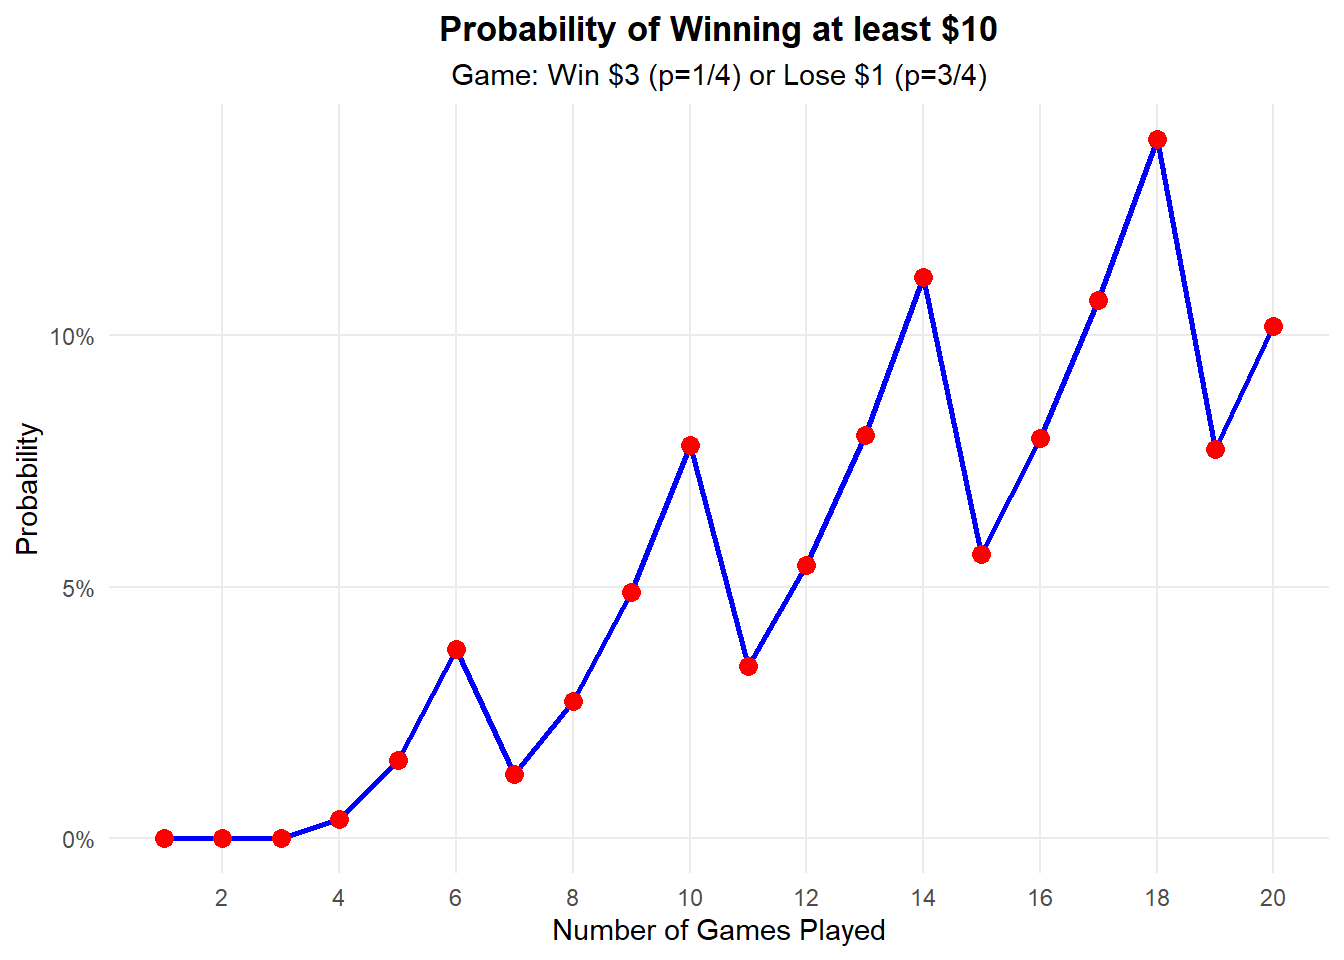
\includegraphics[keepaspectratio]{Assignment_files/figure-latex/unnamed-chunk-2-1.pdf}}

\#\# Assignment 0 Q3

\begin{Shaded}
\begin{Highlighting}[]
\CommentTok{\# Set the range for n}
\NormalTok{n\_values }\OtherTok{\textless{}{-}} \DecValTok{1}\SpecialCharTok{:}\DecValTok{50}

\CommentTok{\# Initialize vectors to store Pn and Qn}
\NormalTok{Pn }\OtherTok{\textless{}{-}} \FunctionTok{numeric}\NormalTok{(}\DecValTok{50}\NormalTok{)}
\NormalTok{Qn }\OtherTok{\textless{}{-}} \FunctionTok{numeric}\NormalTok{(}\DecValTok{50}\NormalTok{)}

\CommentTok{\# Compute Pn and Qn for each n}
\ControlFlowTok{for}\NormalTok{ (n }\ControlFlowTok{in}\NormalTok{ n\_values) \{}
\NormalTok{  m }\OtherTok{\textless{}{-}} \DecValTok{0}\SpecialCharTok{:}\NormalTok{n}
\NormalTok{  P\_HB }\OtherTok{\textless{}{-}} \FunctionTok{dbinom}\NormalTok{(m, n, }\FloatTok{0.5}\NormalTok{)              }\CommentTok{\# P(H\_B = m)}
\NormalTok{  P\_HA\_eq\_m }\OtherTok{\textless{}{-}} \FunctionTok{dbinom}\NormalTok{(m, n}\SpecialCharTok{+}\DecValTok{1}\NormalTok{, }\FloatTok{0.5}\NormalTok{)       }\CommentTok{\# P(H\_A = m)}
\NormalTok{  P\_HA\_gt\_m }\OtherTok{\textless{}{-}} \DecValTok{1} \SpecialCharTok{{-}} \FunctionTok{pbinom}\NormalTok{(m, n}\SpecialCharTok{+}\DecValTok{1}\NormalTok{, }\FloatTok{0.5}\NormalTok{)   }\CommentTok{\# P(H\_A \textgreater{} m)}
\NormalTok{  Qn[n] }\OtherTok{\textless{}{-}} \FunctionTok{sum}\NormalTok{(P\_HB }\SpecialCharTok{*}\NormalTok{ P\_HA\_eq\_m)         }\CommentTok{\# Q\_n = P(H\_A = H\_B)}
\NormalTok{  Pn[n] }\OtherTok{\textless{}{-}} \FunctionTok{sum}\NormalTok{(P\_HB }\SpecialCharTok{*}\NormalTok{ P\_HA\_gt\_m)         }\CommentTok{\# P\_n = P(H\_A \textgreater{} H\_B)}
\NormalTok{\}}

\CommentTok{\# Plot Pn and Qn}
\FunctionTok{plot}\NormalTok{(n\_values, Pn, }\AttributeTok{type=}\StringTok{"l"}\NormalTok{, }\AttributeTok{col=}\StringTok{"blue"}\NormalTok{, }\AttributeTok{ylab=}\StringTok{"Probability"}\NormalTok{, }\AttributeTok{xlab=}\StringTok{"n"}\NormalTok{, }
     \AttributeTok{main=}\StringTok{"Probabilities Pn and Qn for n=1 to 50"}\NormalTok{, }\AttributeTok{ylim=}\FunctionTok{c}\NormalTok{(}\DecValTok{0}\NormalTok{,}\DecValTok{1}\NormalTok{))}
\FunctionTok{lines}\NormalTok{(n\_values, Qn, }\AttributeTok{col=}\StringTok{"red"}\NormalTok{)}
\FunctionTok{legend}\NormalTok{(}\StringTok{"topright"}\NormalTok{, }\AttributeTok{legend=}\FunctionTok{c}\NormalTok{(}\StringTok{"Pn: P(A has more heads than B)"}\NormalTok{, }
                            \StringTok{"Qn: P(A and B have equal heads)"}\NormalTok{), }
       \AttributeTok{col=}\FunctionTok{c}\NormalTok{(}\StringTok{"blue"}\NormalTok{, }\StringTok{"red"}\NormalTok{), }\AttributeTok{lty=}\DecValTok{1}\NormalTok{)}
\end{Highlighting}
\end{Shaded}

\pandocbounded{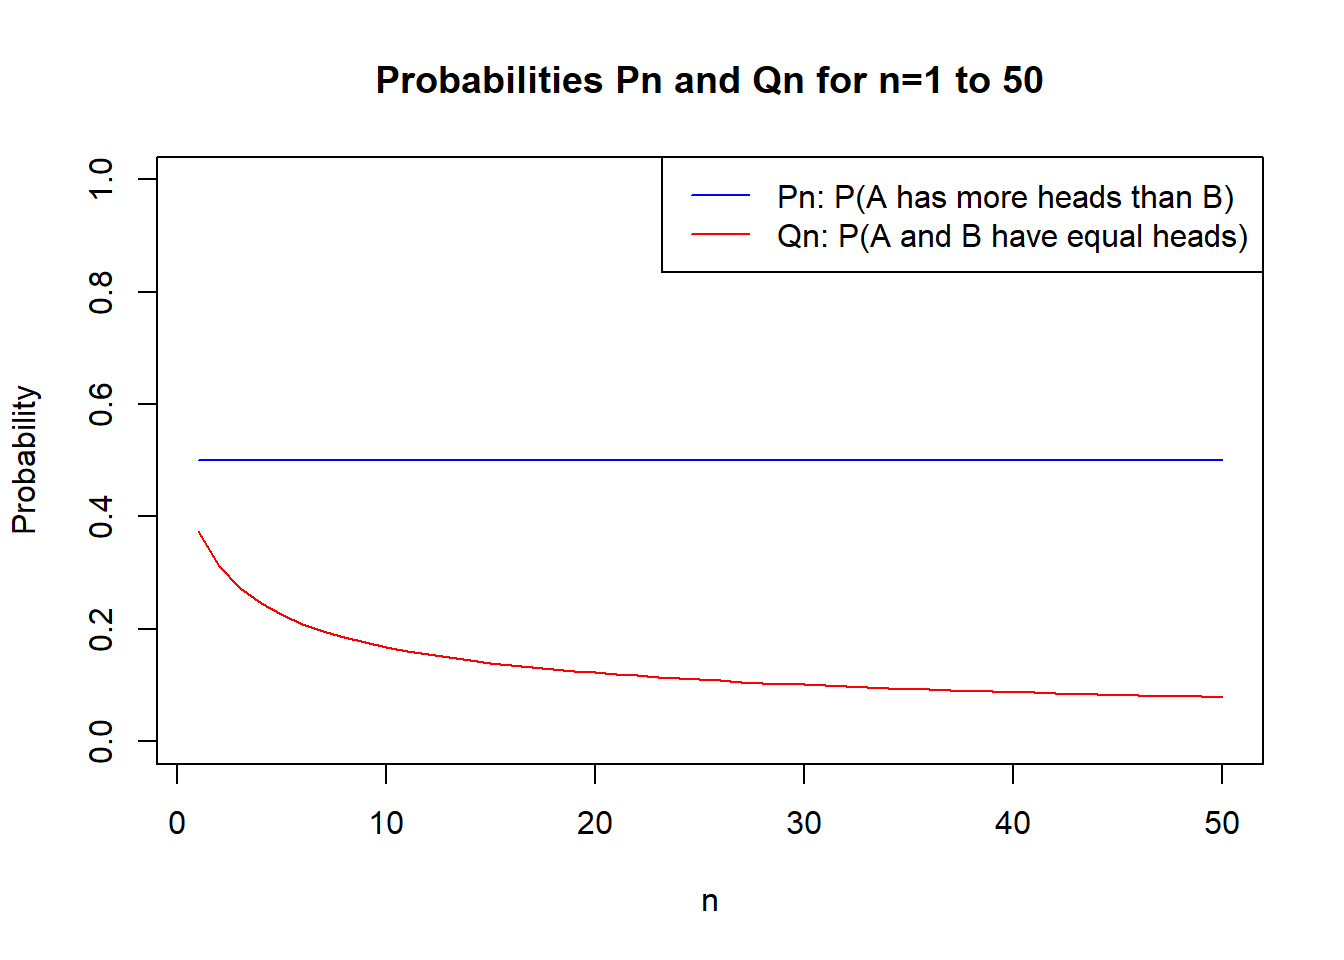
\includegraphics[keepaspectratio]{Assignment_files/figure-latex/unnamed-chunk-3-1.pdf}}

\begin{Shaded}
\begin{Highlighting}[]
\CommentTok{\# Print simple descriptions}
\FunctionTok{cat}\NormalTok{(}\StringTok{"Analysis Results for n = 1 to 50:}\SpecialCharTok{\textbackslash{}n}\StringTok{"}\NormalTok{)}
\end{Highlighting}
\end{Shaded}

\begin{verbatim}
## Analysis Results for n = 1 to 50:
\end{verbatim}

\begin{Shaded}
\begin{Highlighting}[]
\FunctionTok{cat}\NormalTok{(}\StringTok{"Pn is the probability that A, with n+1 coins, has more heads than B, with n coins.}\SpecialCharTok{\textbackslash{}n}\StringTok{"}\NormalTok{)}
\end{Highlighting}
\end{Shaded}

\begin{verbatim}
## Pn is the probability that A, with n+1 coins, has more heads than B, with n coins.
\end{verbatim}

\begin{Shaded}
\begin{Highlighting}[]
\FunctionTok{cat}\NormalTok{(}\StringTok{"Qn is the probability that A and B have an equal number of heads.}\SpecialCharTok{\textbackslash{}n}\StringTok{"}\NormalTok{)}
\end{Highlighting}
\end{Shaded}

\begin{verbatim}
## Qn is the probability that A and B have an equal number of heads.
\end{verbatim}

\begin{Shaded}
\begin{Highlighting}[]
\FunctionTok{cat}\NormalTok{(}\StringTok{"Observations from the computation:}\SpecialCharTok{\textbackslash{}n}\StringTok{"}\NormalTok{)}
\end{Highlighting}
\end{Shaded}

\begin{verbatim}
## Observations from the computation:
\end{verbatim}

\begin{Shaded}
\begin{Highlighting}[]
\FunctionTok{cat}\NormalTok{(}\StringTok{"{-} Pn remains constant at 0.5 for all n from 1 to 50.}\SpecialCharTok{\textbackslash{}n}\StringTok{"}\NormalTok{)}
\end{Highlighting}
\end{Shaded}

\begin{verbatim}
## - Pn remains constant at 0.5 for all n from 1 to 50.
\end{verbatim}

\begin{Shaded}
\begin{Highlighting}[]
\FunctionTok{cat}\NormalTok{(}\StringTok{"{-} Qn decreases as n increases, approaching 0.}\SpecialCharTok{\textbackslash{}n}\StringTok{"}\NormalTok{)}
\end{Highlighting}
\end{Shaded}

\begin{verbatim}
## - Qn decreases as n increases, approaching 0.
\end{verbatim}

\begin{Shaded}
\begin{Highlighting}[]
\FunctionTok{cat}\NormalTok{(}\StringTok{"The plot shows Pn as a blue line and Qn as a red line.}\SpecialCharTok{\textbackslash{}n}\StringTok{"}\NormalTok{)}
\end{Highlighting}
\end{Shaded}

\begin{verbatim}
## The plot shows Pn as a blue line and Qn as a red line.
\end{verbatim}

\#\# Assignment 1 Q1

\begin{Shaded}
\begin{Highlighting}[]
\CommentTok{\# Set parameters}
\NormalTok{epsilon }\OtherTok{\textless{}{-}} \FloatTok{0.01}
\NormalTok{eta }\OtherTok{\textless{}{-}} \FloatTok{0.01}
\NormalTok{p\_values }\OtherTok{\textless{}{-}} \FunctionTok{seq}\NormalTok{(}\FloatTok{0.1}\NormalTok{, }\FloatTok{0.9}\NormalTok{, }\AttributeTok{by =} \FloatTok{0.1}\NormalTok{)}

\CommentTok{\# Calculate minimum n based on the theorem}
\CommentTok{\# n ≥ (1 + ε) / ε\^{}2 * (log(1/η)) + 1/ε}
\NormalTok{calculate\_min\_n }\OtherTok{\textless{}{-}} \ControlFlowTok{function}\NormalTok{(epsilon, eta) \{}
  \FunctionTok{return}\NormalTok{(}\FunctionTok{ceiling}\NormalTok{((}\DecValTok{1} \SpecialCharTok{+}\NormalTok{ epsilon) }\SpecialCharTok{/}\NormalTok{ (epsilon}\SpecialCharTok{\^{}}\DecValTok{2}\NormalTok{) }\SpecialCharTok{*} \FunctionTok{log}\NormalTok{(}\DecValTok{1}\SpecialCharTok{/}\NormalTok{eta) }\SpecialCharTok{+} \DecValTok{1}\SpecialCharTok{/}\NormalTok{epsilon))}
\NormalTok{\}}

\NormalTok{min\_n }\OtherTok{\textless{}{-}} \FunctionTok{calculate\_min\_n}\NormalTok{(epsilon, eta)}
\FunctionTok{cat}\NormalTok{(}\StringTok{"Minimum n from theorem:"}\NormalTok{, min\_n, }\StringTok{"}\SpecialCharTok{\textbackslash{}n}\StringTok{"}\NormalTok{)}
\end{Highlighting}
\end{Shaded}

\begin{verbatim}
## Minimum n from theorem: 46613
\end{verbatim}

\begin{Shaded}
\begin{Highlighting}[]
\CommentTok{\# Calculate exact probabilities using binomial distribution}
\NormalTok{results }\OtherTok{\textless{}{-}} \FunctionTok{data.frame}\NormalTok{(}\AttributeTok{p =}\NormalTok{ p\_values, }\AttributeTok{probability =} \ConstantTok{NA}\NormalTok{, }\AttributeTok{min\_n =} \ConstantTok{NA}\NormalTok{)}

\ControlFlowTok{for}\NormalTok{ (i }\ControlFlowTok{in} \DecValTok{1}\SpecialCharTok{:}\FunctionTok{length}\NormalTok{(p\_values)) \{}
\NormalTok{  p }\OtherTok{\textless{}{-}}\NormalTok{ p\_values[i]}
  
  \CommentTok{\# Calculate the lower and upper bounds for m}
\NormalTok{  lower\_bound }\OtherTok{\textless{}{-}} \FunctionTok{ceiling}\NormalTok{(min\_n }\SpecialCharTok{*}\NormalTok{ (p }\SpecialCharTok{{-}}\NormalTok{ epsilon))}
\NormalTok{  upper\_bound }\OtherTok{\textless{}{-}} \FunctionTok{floor}\NormalTok{(min\_n }\SpecialCharTok{*}\NormalTok{ (p }\SpecialCharTok{+}\NormalTok{ epsilon))}
  
  \CommentTok{\# Adjust bounds to be within [0, n]}
\NormalTok{  adjusted\_lower\_bound }\OtherTok{\textless{}{-}} \FunctionTok{max}\NormalTok{(}\DecValTok{0}\NormalTok{, lower\_bound)}
\NormalTok{  adjusted\_upper\_bound }\OtherTok{\textless{}{-}} \FunctionTok{min}\NormalTok{(min\_n, upper\_bound)}
  
  \CommentTok{\# Calculate probability using pbinom}
  \ControlFlowTok{if}\NormalTok{ (adjusted\_lower\_bound }\SpecialCharTok{\textgreater{}} \DecValTok{0}\NormalTok{) \{}
    \CommentTok{\# P(adjusted\_lower\_bound ≤ X ≤ adjusted\_upper\_bound) = P(X ≤ adjusted\_upper\_bound) {-} P(X ≤ adjusted\_lower\_bound {-} 1)}
\NormalTok{    results}\SpecialCharTok{$}\NormalTok{probability[i] }\OtherTok{\textless{}{-}} \FunctionTok{pbinom}\NormalTok{(adjusted\_upper\_bound, min\_n, p) }\SpecialCharTok{{-}} \FunctionTok{pbinom}\NormalTok{(adjusted\_lower\_bound }\SpecialCharTok{{-}} \DecValTok{1}\NormalTok{, min\_n, p)}
\NormalTok{  \} }\ControlFlowTok{else}\NormalTok{ \{}
    \CommentTok{\# If lower bound is 0, just take P(X ≤ adjusted\_upper\_bound)}
\NormalTok{    results}\SpecialCharTok{$}\NormalTok{probability[i] }\OtherTok{\textless{}{-}} \FunctionTok{pbinom}\NormalTok{(adjusted\_upper\_bound, min\_n, p)}
\NormalTok{  \}}
  
\NormalTok{  results}\SpecialCharTok{$}\NormalTok{min\_n[i] }\OtherTok{\textless{}{-}}\NormalTok{ min\_n}
\NormalTok{\}}

\CommentTok{\# Print results}
\FunctionTok{print}\NormalTok{(results)}
\end{Highlighting}
\end{Shaded}

\begin{verbatim}
##     p probability min_n
## 1 0.1   1.0000000 46613
## 2 0.2   0.9999999 46613
## 3 0.3   0.9999976 46613
## 4 0.4   0.9999895 46613
## 5 0.5   0.9999842 46613
## 6 0.6   0.9999895 46613
## 7 0.7   0.9999976 46613
## 8 0.8   0.9999999 46613
## 9 0.9   1.0000000 46613
\end{verbatim}

\begin{Shaded}
\begin{Highlighting}[]
\FunctionTok{cat}\NormalTok{(}\StringTok{"1 {-} η ="}\NormalTok{, }\DecValTok{1} \SpecialCharTok{{-}}\NormalTok{ eta, }\StringTok{"}\SpecialCharTok{\textbackslash{}n}\StringTok{"}\NormalTok{)}
\end{Highlighting}
\end{Shaded}

\begin{verbatim}
## 1 - η = 0.99
\end{verbatim}

\begin{Shaded}
\begin{Highlighting}[]
\CommentTok{\# Create plot using ggplot2}
\FunctionTok{library}\NormalTok{(ggplot2)}

\CommentTok{\# Add a column for the theoretical bound (1 {-} η)}
\NormalTok{results}\SpecialCharTok{$}\NormalTok{theoretical }\OtherTok{\textless{}{-}} \DecValTok{1} \SpecialCharTok{{-}}\NormalTok{ eta}

\CommentTok{\# Convert to long format for plotting}
\FunctionTok{library}\NormalTok{(tidyr)}
\NormalTok{long\_results }\OtherTok{\textless{}{-}} \FunctionTok{pivot\_longer}\NormalTok{(results, }
                             \AttributeTok{cols =} \FunctionTok{c}\NormalTok{(}\StringTok{"probability"}\NormalTok{, }\StringTok{"theoretical"}\NormalTok{),}
                             \AttributeTok{names\_to =} \StringTok{"type"}\NormalTok{, }
                             \AttributeTok{values\_to =} \StringTok{"value"}\NormalTok{)}

\CommentTok{\# Calculate the range for the "Exact Probability" variable}
\NormalTok{exact\_prob\_range }\OtherTok{\textless{}{-}} \FunctionTok{range}\NormalTok{(results}\SpecialCharTok{$}\NormalTok{probability, }\AttributeTok{na.rm =} \ConstantTok{TRUE}\NormalTok{)}

\CommentTok{\# Plot}
\FunctionTok{ggplot}\NormalTok{(long\_results, }\FunctionTok{aes}\NormalTok{(}\AttributeTok{x =}\NormalTok{ p, }\AttributeTok{y =}\NormalTok{ value, }\AttributeTok{color =}\NormalTok{ type, }\AttributeTok{group =}\NormalTok{ type)) }\SpecialCharTok{+}
  \FunctionTok{geom\_line}\NormalTok{(}\AttributeTok{size =} \DecValTok{1}\NormalTok{) }\SpecialCharTok{+}
  \FunctionTok{geom\_point}\NormalTok{(}\AttributeTok{size =} \DecValTok{3}\NormalTok{) }\SpecialCharTok{+}
  \FunctionTok{scale\_color\_manual}\NormalTok{(}\AttributeTok{values =} \FunctionTok{c}\NormalTok{(}\StringTok{"probability"} \OtherTok{=} \StringTok{"blue"}\NormalTok{, }\StringTok{"theoretical"} \OtherTok{=} \StringTok{"red"}\NormalTok{),}
                    \AttributeTok{labels =} \FunctionTok{c}\NormalTok{(}\StringTok{"probability"} \OtherTok{=} \StringTok{"Exact Probability"}\NormalTok{, }
                              \StringTok{"theoretical"} \OtherTok{=} \StringTok{"Theoretical Bound (1{-}η)"}\NormalTok{)) }\SpecialCharTok{+}
  \FunctionTok{labs}\NormalTok{(}\AttributeTok{title =} \FunctionTok{paste0}\NormalTok{(}\StringTok{"Exact Probability vs Theoretical Bound (1{-}η = "}\NormalTok{, }\DecValTok{1}\SpecialCharTok{{-}}\NormalTok{eta, }\StringTok{")"}\NormalTok{),}
       \AttributeTok{subtitle =} \FunctionTok{paste0}\NormalTok{(}\StringTok{"ε = η = "}\NormalTok{, epsilon, }\StringTok{", n = "}\NormalTok{, min\_n),}
       \AttributeTok{x =} \StringTok{"Success Probability (p)"}\NormalTok{,}
       \AttributeTok{y =} \StringTok{"Probability"}\NormalTok{,}
       \AttributeTok{color =} \StringTok{""}\NormalTok{) }\SpecialCharTok{+}
  \FunctionTok{theme\_minimal}\NormalTok{() }\SpecialCharTok{+}
  \FunctionTok{theme}\NormalTok{(}\AttributeTok{legend.position =} \StringTok{"bottom"}\NormalTok{) }\SpecialCharTok{+}
  \FunctionTok{ylim}\NormalTok{(exact\_prob\_range[}\DecValTok{1}\NormalTok{], exact\_prob\_range[}\DecValTok{2}\NormalTok{])}
\end{Highlighting}
\end{Shaded}

\begin{verbatim}
## Warning: Removed 9 rows containing missing values or values outside the scale range
## (`geom_line()`).
\end{verbatim}

\begin{verbatim}
## Warning: Removed 9 rows containing missing values or values outside the scale range
## (`geom_point()`).
\end{verbatim}

\pandocbounded{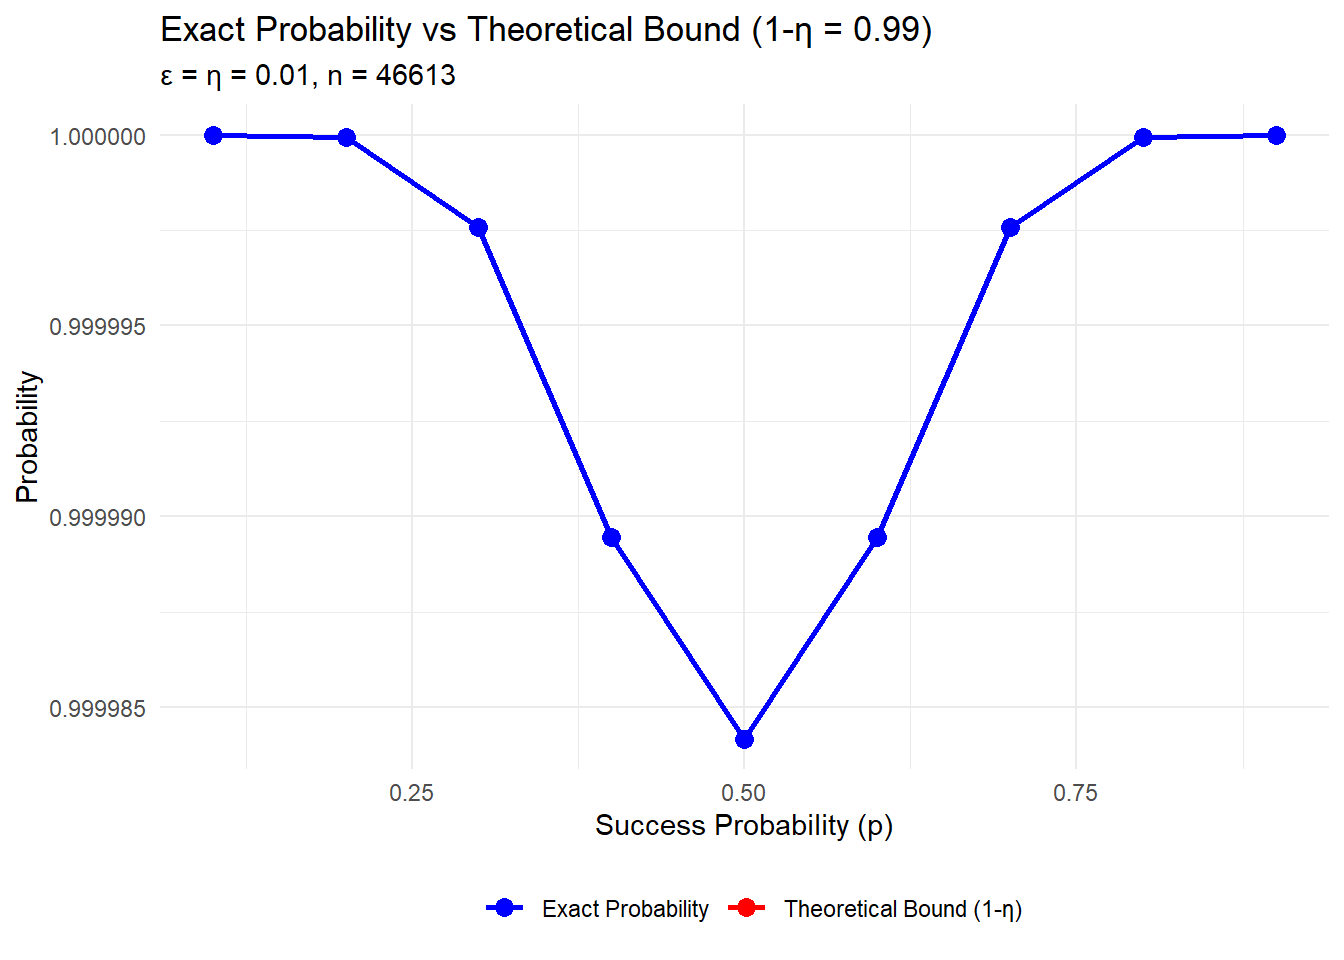
\includegraphics[keepaspectratio]{Assignment_files/figure-latex/unnamed-chunk-4-1.pdf}}

\#\# Assignment 1 Q2

\begin{Shaded}
\begin{Highlighting}[]
\CommentTok{\# Load required libraries}
\FunctionTok{library}\NormalTok{(dplyr)      }\CommentTok{\# For data manipulation}
\end{Highlighting}
\end{Shaded}

\begin{verbatim}
## 
## Attaching package: 'dplyr'
\end{verbatim}

\begin{verbatim}
## The following objects are masked from 'package:stats':
## 
##     filter, lag
\end{verbatim}

\begin{verbatim}
## The following objects are masked from 'package:base':
## 
##     intersect, setdiff, setequal, union
\end{verbatim}

\begin{Shaded}
\begin{Highlighting}[]
\FunctionTok{library}\NormalTok{(ggplot2)    }\CommentTok{\# For plotting}
\FunctionTok{library}\NormalTok{(lubridate)  }\CommentTok{\# For date handling}
\end{Highlighting}
\end{Shaded}

\begin{verbatim}
## 
## Attaching package: 'lubridate'
\end{verbatim}

\begin{verbatim}
## The following objects are masked from 'package:base':
## 
##     date, intersect, setdiff, union
\end{verbatim}

\begin{Shaded}
\begin{Highlighting}[]
\CommentTok{\# Read the CPI data from a CSV file}
\NormalTok{cpi\_data }\OtherTok{\textless{}{-}} \FunctionTok{read.csv}\NormalTok{(}\StringTok{"cpi.csv"}\NormalTok{, }\AttributeTok{header =} \ConstantTok{TRUE}\NormalTok{)}

\CommentTok{\# Filter to keep only monthly data (exclude rows where Month is missing or empty)}
\NormalTok{monthly\_data }\OtherTok{\textless{}{-}}\NormalTok{ cpi\_data[}\SpecialCharTok{!}\FunctionTok{is.na}\NormalTok{(cpi\_data}\SpecialCharTok{$}\NormalTok{Month) }\SpecialCharTok{\&}\NormalTok{ cpi\_data}\SpecialCharTok{$}\NormalTok{Month }\SpecialCharTok{!=} \StringTok{""}\NormalTok{, ]}

\CommentTok{\# Convert Month to a factor with calendar order}
\NormalTok{monthly\_data}\SpecialCharTok{$}\NormalTok{Month }\OtherTok{\textless{}{-}} \FunctionTok{factor}\NormalTok{(monthly\_data}\SpecialCharTok{$}\NormalTok{Month, }
                             \AttributeTok{levels =} \FunctionTok{c}\NormalTok{(}\StringTok{"Jan"}\NormalTok{, }\StringTok{"Feb"}\NormalTok{, }\StringTok{"Mar"}\NormalTok{, }\StringTok{"Apr"}\NormalTok{, }\StringTok{"May"}\NormalTok{, }\StringTok{"Jun"}\NormalTok{, }
                                        \StringTok{"Jul"}\NormalTok{, }\StringTok{"Aug"}\NormalTok{, }\StringTok{"Sep"}\NormalTok{, }\StringTok{"Oct"}\NormalTok{, }\StringTok{"Nov"}\NormalTok{, }\StringTok{"Dec"}\NormalTok{))}

\CommentTok{\# Create a Date column for easier date{-}based filtering}
\NormalTok{monthly\_data}\SpecialCharTok{$}\NormalTok{Date }\OtherTok{\textless{}{-}} \FunctionTok{as.Date}\NormalTok{(}\FunctionTok{paste}\NormalTok{(monthly\_data}\SpecialCharTok{$}\NormalTok{Year, }\FunctionTok{match}\NormalTok{(monthly\_data}\SpecialCharTok{$}\NormalTok{Month, month.abb), }\StringTok{"01"}\NormalTok{, }\AttributeTok{sep =} \StringTok{"{-}"}\NormalTok{), }
                             \AttributeTok{format =} \StringTok{"\%Y{-}\%m{-}\%d"}\NormalTok{)}

\CommentTok{\# Sort the data by Date}
\NormalTok{monthly\_data }\OtherTok{\textless{}{-}}\NormalTok{ monthly\_data }\SpecialCharTok{\%\textgreater{}\%} \FunctionTok{arrange}\NormalTok{(Date)}

\CommentTok{\# Function to calculate H1 and H2 for each year}
\NormalTok{calculate\_H1\_H2 }\OtherTok{\textless{}{-}} \ControlFlowTok{function}\NormalTok{(data) \{}
  \CommentTok{\# Initialize lists to store H1 and H2 values}
\NormalTok{  H1\_list }\OtherTok{\textless{}{-}} \FunctionTok{list}\NormalTok{()}
\NormalTok{  H2\_list }\OtherTok{\textless{}{-}} \FunctionTok{list}\NormalTok{()}
  
  \CommentTok{\# Get unique years in the dataset}
\NormalTok{  years }\OtherTok{\textless{}{-}} \FunctionTok{unique}\NormalTok{(}\FunctionTok{year}\NormalTok{(data}\SpecialCharTok{$}\NormalTok{Date))}
  
  \ControlFlowTok{for}\NormalTok{ (yr }\ControlFlowTok{in}\NormalTok{ years) \{}
    \CommentTok{\# H1: Average CPI from May to October of the current year}
\NormalTok{    start\_H1 }\OtherTok{\textless{}{-}} \FunctionTok{as.Date}\NormalTok{(}\FunctionTok{paste}\NormalTok{(yr, }\StringTok{"05{-}01"}\NormalTok{, }\AttributeTok{sep =} \StringTok{"{-}"}\NormalTok{))}
\NormalTok{    end\_H1 }\OtherTok{\textless{}{-}} \FunctionTok{as.Date}\NormalTok{(}\FunctionTok{paste}\NormalTok{(yr, }\StringTok{"10{-}01"}\NormalTok{, }\AttributeTok{sep =} \StringTok{"{-}"}\NormalTok{))}
\NormalTok{    H1\_data }\OtherTok{\textless{}{-}}\NormalTok{ data }\SpecialCharTok{\%\textgreater{}\%} \FunctionTok{filter}\NormalTok{(Date }\SpecialCharTok{\textgreater{}=}\NormalTok{ start\_H1 }\SpecialCharTok{\&}\NormalTok{ Date }\SpecialCharTok{\textless{}=}\NormalTok{ end\_H1)}
    \ControlFlowTok{if}\NormalTok{ (}\FunctionTok{nrow}\NormalTok{(H1\_data) }\SpecialCharTok{==} \DecValTok{6}\NormalTok{) \{  }\CommentTok{\# Ensure exactly 6 months of data}
\NormalTok{      H1\_list[[}\FunctionTok{as.character}\NormalTok{(yr)]] }\OtherTok{\textless{}{-}} \FunctionTok{mean}\NormalTok{(H1\_data}\SpecialCharTok{$}\NormalTok{CPI)}
\NormalTok{    \}}
    
    \CommentTok{\# H2: Average CPI from November of the current year to April of the next year}
\NormalTok{    start\_H2 }\OtherTok{\textless{}{-}} \FunctionTok{as.Date}\NormalTok{(}\FunctionTok{paste}\NormalTok{(yr, }\StringTok{"11{-}01"}\NormalTok{, }\AttributeTok{sep =} \StringTok{"{-}"}\NormalTok{))}
\NormalTok{    end\_H2 }\OtherTok{\textless{}{-}} \FunctionTok{as.Date}\NormalTok{(}\FunctionTok{paste}\NormalTok{(yr }\SpecialCharTok{+} \DecValTok{1}\NormalTok{, }\StringTok{"04{-}01"}\NormalTok{, }\AttributeTok{sep =} \StringTok{"{-}"}\NormalTok{))}
\NormalTok{    H2\_data }\OtherTok{\textless{}{-}}\NormalTok{ data }\SpecialCharTok{\%\textgreater{}\%} \FunctionTok{filter}\NormalTok{(Date }\SpecialCharTok{\textgreater{}=}\NormalTok{ start\_H2 }\SpecialCharTok{\&}\NormalTok{ Date }\SpecialCharTok{\textless{}=}\NormalTok{ end\_H2)}
    \ControlFlowTok{if}\NormalTok{ (}\FunctionTok{nrow}\NormalTok{(H2\_data) }\SpecialCharTok{==} \DecValTok{6}\NormalTok{) \{  }\CommentTok{\# Ensure exactly 6 months of data}
\NormalTok{      H2\_list[[}\FunctionTok{as.character}\NormalTok{(yr)]] }\OtherTok{\textless{}{-}} \FunctionTok{mean}\NormalTok{(H2\_data}\SpecialCharTok{$}\NormalTok{CPI)}
\NormalTok{    \}}
\NormalTok{  \}}
  
  \CommentTok{\# Convert lists to data frames}
\NormalTok{  H1\_df }\OtherTok{\textless{}{-}} \FunctionTok{data.frame}\NormalTok{(}\AttributeTok{Year =} \FunctionTok{as.integer}\NormalTok{(}\FunctionTok{names}\NormalTok{(H1\_list)), }\AttributeTok{H1 =} \FunctionTok{unlist}\NormalTok{(H1\_list))}
\NormalTok{  H2\_df }\OtherTok{\textless{}{-}} \FunctionTok{data.frame}\NormalTok{(}\AttributeTok{Year =} \FunctionTok{as.integer}\NormalTok{(}\FunctionTok{names}\NormalTok{(H2\_list)), }\AttributeTok{H2 =} \FunctionTok{unlist}\NormalTok{(H2\_list))}
  
  \FunctionTok{return}\NormalTok{(}\FunctionTok{list}\NormalTok{(}\AttributeTok{H1 =}\NormalTok{ H1\_df, }\AttributeTok{H2 =}\NormalTok{ H2\_df))}
\NormalTok{\}}

\CommentTok{\# Calculate H1 and H2}
\NormalTok{H1\_H2 }\OtherTok{\textless{}{-}} \FunctionTok{calculate\_H1\_H2}\NormalTok{(monthly\_data)}

\CommentTok{\# Merge H1 and H2 into a single data frame for plotting}
\NormalTok{H1\_H2\_df }\OtherTok{\textless{}{-}} \FunctionTok{full\_join}\NormalTok{(H1\_H2}\SpecialCharTok{$}\NormalTok{H1, H1\_H2}\SpecialCharTok{$}\NormalTok{H2, }\AttributeTok{by =} \StringTok{"Year"}\NormalTok{)}

\CommentTok{\# Create the line plot}
\FunctionTok{ggplot}\NormalTok{(H1\_H2\_df, }\FunctionTok{aes}\NormalTok{(}\AttributeTok{x =}\NormalTok{ Year)) }\SpecialCharTok{+}
  \FunctionTok{geom\_line}\NormalTok{(}\FunctionTok{aes}\NormalTok{(}\AttributeTok{y =}\NormalTok{ H1, }\AttributeTok{color =} \StringTok{"H1"}\NormalTok{)) }\SpecialCharTok{+}  \CommentTok{\# H1 in blue}
  \FunctionTok{geom\_line}\NormalTok{(}\FunctionTok{aes}\NormalTok{(}\AttributeTok{y =}\NormalTok{ H2, }\AttributeTok{color =} \StringTok{"H2"}\NormalTok{)) }\SpecialCharTok{+}  \CommentTok{\# H2 in red}
  \FunctionTok{labs}\NormalTok{(}\AttributeTok{title =} \StringTok{"Time Series of H1 and H2"}\NormalTok{,}
       \AttributeTok{x =} \StringTok{"Year"}\NormalTok{,}
       \AttributeTok{y =} \StringTok{"Average CPI"}\NormalTok{) }\SpecialCharTok{+}
  \FunctionTok{scale\_color\_manual}\NormalTok{(}\AttributeTok{values =} \FunctionTok{c}\NormalTok{(}\StringTok{"H1"} \OtherTok{=} \StringTok{"blue"}\NormalTok{, }\StringTok{"H2"} \OtherTok{=} \StringTok{"red"}\NormalTok{),}
                     \AttributeTok{name =} \StringTok{"Series"}\NormalTok{) }\SpecialCharTok{+}
  \FunctionTok{theme\_minimal}\NormalTok{()}
\end{Highlighting}
\end{Shaded}

\begin{verbatim}
## Warning: Removed 1 row containing missing values or values outside the scale range
## (`geom_line()`).
\end{verbatim}

\pandocbounded{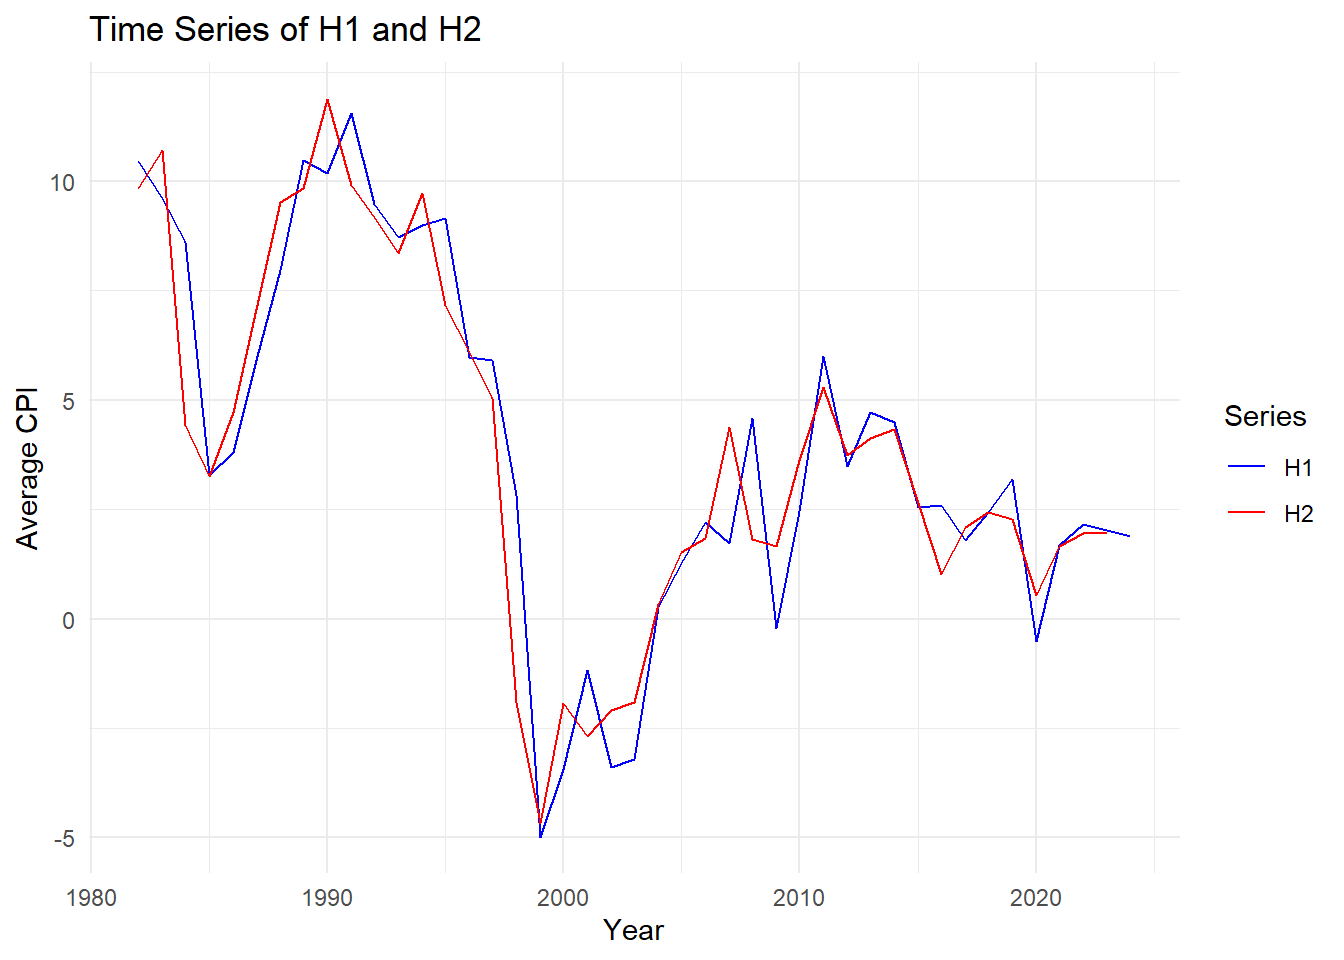
\includegraphics[keepaspectratio]{Assignment_files/figure-latex/unnamed-chunk-5-1.pdf}}

Assignment 1 Q3

\begin{Shaded}
\begin{Highlighting}[]
  \CommentTok{\# Load necessary libraries}
\FunctionTok{library}\NormalTok{(ggplot2)}

\CommentTok{\# Define the cash flow dates and values}
\NormalTok{dates }\OtherTok{\textless{}{-}} \FunctionTok{as.Date}\NormalTok{(}\FunctionTok{c}\NormalTok{(}\StringTok{"2023{-}06{-}01"}\NormalTok{, }\StringTok{"2023{-}07{-}26"}\NormalTok{, }\StringTok{"2023{-}08{-}29"}\NormalTok{, }\StringTok{"2023{-}09{-}01"}\NormalTok{))}
\NormalTok{base\_flows }\OtherTok{\textless{}{-}} \FunctionTok{c}\NormalTok{(}\DecValTok{0}\NormalTok{, }\SpecialCharTok{{-}}\FloatTok{1873.9}\NormalTok{, }\SpecialCharTok{{-}}\FloatTok{39767.0}\NormalTok{, }\ConstantTok{NA}\NormalTok{)  }\CommentTok{\# Last value will depend on exchange rate}

\CommentTok{\# Function to calculate days between dates}
\NormalTok{days\_between }\OtherTok{\textless{}{-}} \ControlFlowTok{function}\NormalTok{(start\_date, end\_date) \{}
  \FunctionTok{as.numeric}\NormalTok{(}\FunctionTok{difftime}\NormalTok{(end\_date, start\_date, }\AttributeTok{units =} \StringTok{"days"}\NormalTok{))}
\NormalTok{\}}

\CommentTok{\# Calculate time intervals in years (using day count)}
\NormalTok{t0 }\OtherTok{\textless{}{-}}\NormalTok{ dates[}\DecValTok{1}\NormalTok{]}
\NormalTok{time\_intervals }\OtherTok{\textless{}{-}} \FunctionTok{days\_between}\NormalTok{(t0, dates) }\SpecialCharTok{/} \DecValTok{365}

\CommentTok{\# Function to calculate NPV given a rate and cash flows}
\NormalTok{npv\_func }\OtherTok{\textless{}{-}} \ControlFlowTok{function}\NormalTok{(rate, cashflows, timepoints) \{}
  \FunctionTok{sum}\NormalTok{(cashflows }\SpecialCharTok{/}\NormalTok{ (}\DecValTok{1} \SpecialCharTok{+}\NormalTok{ rate)}\SpecialCharTok{\^{}}\NormalTok{timepoints)}
\NormalTok{\}}

\CommentTok{\# Function to find IRR for a specific exchange rate}
\NormalTok{find\_irr }\OtherTok{\textless{}{-}} \ControlFlowTok{function}\NormalTok{(xr) \{}
  \CommentTok{\# Calculate the final cash flow based on exchange rate}
\NormalTok{  final\_flow }\OtherTok{\textless{}{-}} \FloatTok{193518.2} \SpecialCharTok{*}\NormalTok{ xr }\SpecialCharTok{{-}} \DecValTok{1465686}
  
  \CommentTok{\# Complete cash flows vector}
\NormalTok{  cash\_flows }\OtherTok{\textless{}{-}} \FunctionTok{c}\NormalTok{(base\_flows[}\DecValTok{1}\SpecialCharTok{:}\DecValTok{3}\NormalTok{], final\_flow)}
  
  \CommentTok{\# Function to find the root of (for uniroot)}
\NormalTok{  f }\OtherTok{\textless{}{-}} \ControlFlowTok{function}\NormalTok{(r) }\FunctionTok{npv\_func}\NormalTok{(r, cash\_flows, time\_intervals)}
  
  \CommentTok{\# Use uniroot to find IRR}
\NormalTok{  result }\OtherTok{\textless{}{-}} \FunctionTok{tryCatch}\NormalTok{(\{}
    \FunctionTok{uniroot}\NormalTok{(f, }\AttributeTok{interval =} \FunctionTok{c}\NormalTok{(}\SpecialCharTok{{-}}\FloatTok{0.9999}\NormalTok{, }\FloatTok{1.0}\NormalTok{), }\AttributeTok{extendInt =} \StringTok{"yes"}\NormalTok{)}
\NormalTok{  \}, }\AttributeTok{error =} \ControlFlowTok{function}\NormalTok{(e) \{}
    \FunctionTok{return}\NormalTok{(}\FunctionTok{list}\NormalTok{(}\AttributeTok{root =} \ConstantTok{NA}\NormalTok{))}
\NormalTok{  \})}
  
  \FunctionTok{return}\NormalTok{(result}\SpecialCharTok{$}\NormalTok{root)}
\NormalTok{\}}

\CommentTok{\# Generate sequence of exchange rates}
\NormalTok{exchange\_rates }\OtherTok{\textless{}{-}} \FunctionTok{seq}\NormalTok{(}\FloatTok{7.75}\NormalTok{, }\FloatTok{7.85}\NormalTok{, }\AttributeTok{by =} \FloatTok{0.005}\NormalTok{)}

\CommentTok{\# Calculate IRR for each exchange rate}
\NormalTok{irr\_values }\OtherTok{\textless{}{-}} \FunctionTok{sapply}\NormalTok{(exchange\_rates, find\_irr)}

\CommentTok{\# Create a data frame for plotting}
\NormalTok{results }\OtherTok{\textless{}{-}} \FunctionTok{data.frame}\NormalTok{(}
  \AttributeTok{ExchangeRate =}\NormalTok{ exchange\_rates,}
  \AttributeTok{IRR =}\NormalTok{ irr\_values}
\NormalTok{)}

\CommentTok{\# Print results table}
\FunctionTok{print}\NormalTok{(results)}
\end{Highlighting}
\end{Shaded}

\begin{verbatim}
##    ExchangeRate           IRR
## 1         7.750 -9.999219e-01
## 2         7.755 -1.000000e+00
## 3         7.760 -9.999989e-01
## 4         7.765 -9.999256e-01
## 5         7.770 -9.997720e-01
## 6         7.775 -9.972420e-01
## 7         7.780 -9.740206e-01
## 8         7.785 -7.928617e-01
## 9         7.790  4.126901e-01
## 10        7.795  7.319670e+00
## 11        7.800  4.177278e+01
## 12        7.805  1.931534e+02
## 13        7.810  7.858445e+02
## 14        7.815  2.876638e+03
## 15        7.820  9.591108e+03
## 16        7.825  2.940869e+04
## 17        7.830  8.362839e+04
## 18        7.835  2.221996e+05
## 19        7.840  5.553003e+05
## 20        7.845  1.313013e+06
## 21        7.850  2.952836e+06
\end{verbatim}

\begin{Shaded}
\begin{Highlighting}[]
\CommentTok{\# Plot the IRR against exchange rates}
\NormalTok{p }\OtherTok{\textless{}{-}} \FunctionTok{ggplot}\NormalTok{(results, }\FunctionTok{aes}\NormalTok{(}\AttributeTok{x =}\NormalTok{ ExchangeRate, }\AttributeTok{y =}\NormalTok{ IRR)) }\SpecialCharTok{+}
  \FunctionTok{geom\_line}\NormalTok{(}\AttributeTok{color =} \StringTok{"blue"}\NormalTok{, }\AttributeTok{size =} \DecValTok{1}\NormalTok{) }\SpecialCharTok{+}
  \FunctionTok{geom\_point}\NormalTok{(}\AttributeTok{color =} \StringTok{"red"}\NormalTok{, }\AttributeTok{size =} \DecValTok{2}\NormalTok{) }\SpecialCharTok{+}
  \FunctionTok{labs}\NormalTok{(}
    \AttributeTok{title =} \StringTok{"IRR vs USD/HKD Exchange Rate"}\NormalTok{,}
    \AttributeTok{x =} \StringTok{"USD/HKD Exchange Rate"}\NormalTok{,}
    \AttributeTok{y =} \StringTok{"Internal Rate of Return (IRR)"}\NormalTok{,}
    \AttributeTok{caption =} \StringTok{"Step size: 0.005"}
\NormalTok{  ) }\SpecialCharTok{+}
  \FunctionTok{theme\_minimal}\NormalTok{() }\SpecialCharTok{+}
  \FunctionTok{scale\_y\_continuous}\NormalTok{(}\AttributeTok{labels =}\NormalTok{ scales}\SpecialCharTok{::}\NormalTok{percent) }\SpecialCharTok{+}
  \FunctionTok{geom\_hline}\NormalTok{(}\AttributeTok{yintercept =} \DecValTok{0}\NormalTok{, }\AttributeTok{linetype =} \StringTok{"dashed"}\NormalTok{, }\AttributeTok{color =} \StringTok{"darkgray"}\NormalTok{) }\SpecialCharTok{+}
  \FunctionTok{theme}\NormalTok{(}
    \AttributeTok{plot.title =} \FunctionTok{element\_text}\NormalTok{(}\AttributeTok{hjust =} \FloatTok{0.5}\NormalTok{, }\AttributeTok{face =} \StringTok{"bold"}\NormalTok{),}
    \AttributeTok{axis.title =} \FunctionTok{element\_text}\NormalTok{(}\AttributeTok{face =} \StringTok{"bold"}\NormalTok{)}
\NormalTok{  )}

\CommentTok{\# Display the plot}
\FunctionTok{print}\NormalTok{(p)}
\end{Highlighting}
\end{Shaded}

\pandocbounded{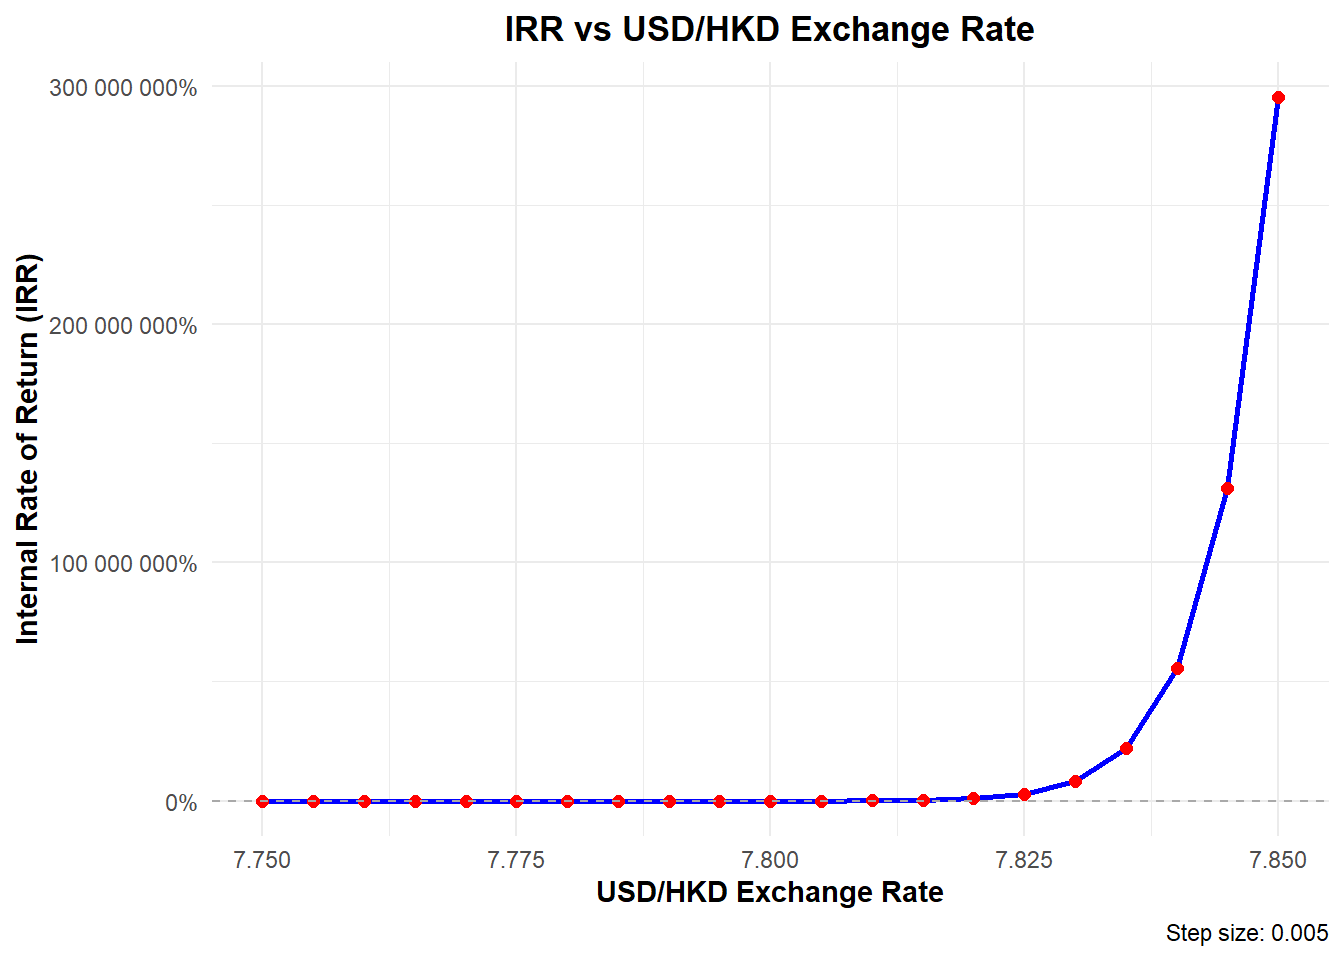
\includegraphics[keepaspectratio]{Assignment_files/figure-latex/unnamed-chunk-6-1.pdf}}

\begin{Shaded}
\begin{Highlighting}[]
\CommentTok{\# Save plot to file if needed}
\CommentTok{\# ggsave("irr\_vs\_exchange\_rate.png", p, width = 10, height = 6, dpi = 300)}
\end{Highlighting}
\end{Shaded}

\#\# Assignment 1 Q4

\begin{Shaded}
\begin{Highlighting}[]
\CommentTok{\# Analysis of uncertain cash flows using Hazen (2009) mean decision rule}

\CommentTok{\# Set the discount rate}
\NormalTok{discount\_rate }\OtherTok{\textless{}{-}} \FloatTok{0.06}

\CommentTok{\# Define initial investment}
\NormalTok{C0 }\OtherTok{\textless{}{-}} \SpecialCharTok{{-}}\DecValTok{100}

\CommentTok{\# Define possible paths and their probabilities}
\CommentTok{\# Path 1: C0 {-}\textgreater{} C1(70) {-}\textgreater{} C2(80)}
\CommentTok{\# Path 2: C0 {-}\textgreater{} C1(70) {-}\textgreater{} C2(50)}
\CommentTok{\# Path 3: C0 {-}\textgreater{} C1(50) {-}\textgreater{} C2(50)}

\CommentTok{\# Calculate NPV for each path}
\CommentTok{\# Path 1: C0 {-}\textgreater{} C1(70) {-}\textgreater{} C2(80) with probability 0.4 * 0.2 = 0.08}
\NormalTok{path1\_cf }\OtherTok{\textless{}{-}} \FunctionTok{c}\NormalTok{(C0, }\DecValTok{70}\NormalTok{, }\DecValTok{80}\NormalTok{)}
\NormalTok{path1\_npv }\OtherTok{\textless{}{-}}\NormalTok{ path1\_cf[}\DecValTok{1}\NormalTok{] }\SpecialCharTok{+} 
\NormalTok{             path1\_cf[}\DecValTok{2}\NormalTok{] }\SpecialCharTok{/}\NormalTok{ (}\DecValTok{1} \SpecialCharTok{+}\NormalTok{ discount\_rate)}\SpecialCharTok{\^{}}\DecValTok{1} \SpecialCharTok{+} 
\NormalTok{             path1\_cf[}\DecValTok{3}\NormalTok{] }\SpecialCharTok{/}\NormalTok{ (}\DecValTok{1} \SpecialCharTok{+}\NormalTok{ discount\_rate)}\SpecialCharTok{\^{}}\DecValTok{2}
\NormalTok{path1\_prob }\OtherTok{\textless{}{-}} \FloatTok{0.4} \SpecialCharTok{*} \FloatTok{0.2}

\CommentTok{\# Path 2: C0 {-}\textgreater{} C1(70) {-}\textgreater{} C2(50) with probability 0.4 * 0.8 = 0.32}
\NormalTok{path2\_cf }\OtherTok{\textless{}{-}} \FunctionTok{c}\NormalTok{(C0, }\DecValTok{70}\NormalTok{, }\DecValTok{50}\NormalTok{)}
\NormalTok{path2\_npv }\OtherTok{\textless{}{-}}\NormalTok{ path2\_cf[}\DecValTok{1}\NormalTok{] }\SpecialCharTok{+} 
\NormalTok{             path2\_cf[}\DecValTok{2}\NormalTok{] }\SpecialCharTok{/}\NormalTok{ (}\DecValTok{1} \SpecialCharTok{+}\NormalTok{ discount\_rate)}\SpecialCharTok{\^{}}\DecValTok{1} \SpecialCharTok{+} 
\NormalTok{             path2\_cf[}\DecValTok{3}\NormalTok{] }\SpecialCharTok{/}\NormalTok{ (}\DecValTok{1} \SpecialCharTok{+}\NormalTok{ discount\_rate)}\SpecialCharTok{\^{}}\DecValTok{2}
\NormalTok{path2\_prob }\OtherTok{\textless{}{-}} \FloatTok{0.4} \SpecialCharTok{*} \FloatTok{0.8}

\CommentTok{\# Path 3: C0 {-}\textgreater{} C1(50) {-}\textgreater{} C2(50) with probability 0.6 * 1.0 = 0.6}
\NormalTok{path3\_cf }\OtherTok{\textless{}{-}} \FunctionTok{c}\NormalTok{(C0, }\DecValTok{50}\NormalTok{, }\DecValTok{50}\NormalTok{)}
\NormalTok{path3\_npv }\OtherTok{\textless{}{-}}\NormalTok{ path3\_cf[}\DecValTok{1}\NormalTok{] }\SpecialCharTok{+} 
\NormalTok{             path3\_cf[}\DecValTok{2}\NormalTok{] }\SpecialCharTok{/}\NormalTok{ (}\DecValTok{1} \SpecialCharTok{+}\NormalTok{ discount\_rate)}\SpecialCharTok{\^{}}\DecValTok{1} \SpecialCharTok{+} 
\NormalTok{             path3\_cf[}\DecValTok{3}\NormalTok{] }\SpecialCharTok{/}\NormalTok{ (}\DecValTok{1} \SpecialCharTok{+}\NormalTok{ discount\_rate)}\SpecialCharTok{\^{}}\DecValTok{2}
\NormalTok{path3\_prob }\OtherTok{\textless{}{-}} \FloatTok{0.6} \SpecialCharTok{*} \FloatTok{1.0}

\CommentTok{\# Create a summary table for paths}
\NormalTok{paths\_df }\OtherTok{\textless{}{-}} \FunctionTok{data.frame}\NormalTok{(}
  \AttributeTok{Path =} \FunctionTok{c}\NormalTok{(}\StringTok{"Path 1: C0 {-}\textgreater{} C1(70) {-}\textgreater{} C2(80)"}\NormalTok{, }
           \StringTok{"Path 2: C0 {-}\textgreater{} C1(70) {-}\textgreater{} C2(50)"}\NormalTok{, }
           \StringTok{"Path 3: C0 {-}\textgreater{} C1(50) {-}\textgreater{} C2(50)"}\NormalTok{),}
  \AttributeTok{Probability =} \FunctionTok{c}\NormalTok{(path1\_prob, path2\_prob, path3\_prob),}
  \AttributeTok{NPV =} \FunctionTok{c}\NormalTok{(path1\_npv, path2\_npv, path3\_npv)}
\NormalTok{)}

\CommentTok{\# Calculate expected NPV using Hazen\textquotesingle{}s mean decision rule}
\NormalTok{expected\_npv }\OtherTok{\textless{}{-}}\NormalTok{ path1\_prob }\SpecialCharTok{*}\NormalTok{ path1\_npv }\SpecialCharTok{+} 
\NormalTok{                path2\_prob }\SpecialCharTok{*}\NormalTok{ path2\_npv }\SpecialCharTok{+} 
\NormalTok{                path3\_prob }\SpecialCharTok{*}\NormalTok{ path3\_npv}

\CommentTok{\# Print results}
\FunctionTok{cat}\NormalTok{(}\StringTok{"Hazen (2009) Mean Decision Rule Analysis}\SpecialCharTok{\textbackslash{}n}\StringTok{"}\NormalTok{)}
\end{Highlighting}
\end{Shaded}

\begin{verbatim}
## Hazen (2009) Mean Decision Rule Analysis
\end{verbatim}

\begin{Shaded}
\begin{Highlighting}[]
\FunctionTok{cat}\NormalTok{(}\StringTok{"========================================}\SpecialCharTok{\textbackslash{}n\textbackslash{}n}\StringTok{"}\NormalTok{)}
\end{Highlighting}
\end{Shaded}

\begin{verbatim}
## ========================================
\end{verbatim}

\begin{Shaded}
\begin{Highlighting}[]
\FunctionTok{cat}\NormalTok{(}\StringTok{"Discount Rate:"}\NormalTok{, discount\_rate }\SpecialCharTok{*} \DecValTok{100}\NormalTok{, }\StringTok{"\%}\SpecialCharTok{\textbackslash{}n\textbackslash{}n}\StringTok{"}\NormalTok{)}
\end{Highlighting}
\end{Shaded}

\begin{verbatim}
## Discount Rate: 6 %
\end{verbatim}

\begin{Shaded}
\begin{Highlighting}[]
\FunctionTok{cat}\NormalTok{(}\StringTok{"NPV Calculation for Each Path:}\SpecialCharTok{\textbackslash{}n}\StringTok{"}\NormalTok{)}
\end{Highlighting}
\end{Shaded}

\begin{verbatim}
## NPV Calculation for Each Path:
\end{verbatim}

\begin{Shaded}
\begin{Highlighting}[]
\FunctionTok{print}\NormalTok{(paths\_df, }\AttributeTok{row.names =} \ConstantTok{FALSE}\NormalTok{)}
\end{Highlighting}
\end{Shaded}

\begin{verbatim}
##                            Path Probability       NPV
##  Path 1: C0 -> C1(70) -> C2(80)        0.08 37.237451
##  Path 2: C0 -> C1(70) -> C2(50)        0.32 10.537558
##  Path 3: C0 -> C1(50) -> C2(50)        0.60 -8.330367
\end{verbatim}

\begin{Shaded}
\begin{Highlighting}[]
\FunctionTok{cat}\NormalTok{(}\StringTok{"}\SpecialCharTok{\textbackslash{}n}\StringTok{"}\NormalTok{)}
\end{Highlighting}
\end{Shaded}

\begin{Shaded}
\begin{Highlighting}[]
\FunctionTok{cat}\NormalTok{(}\StringTok{"Expected NPV:"}\NormalTok{, }\FunctionTok{round}\NormalTok{(expected\_npv, }\DecValTok{2}\NormalTok{), }\StringTok{"}\SpecialCharTok{\textbackslash{}n\textbackslash{}n}\StringTok{"}\NormalTok{)}
\end{Highlighting}
\end{Shaded}

\begin{verbatim}
## Expected NPV: 1.35
\end{verbatim}

\begin{Shaded}
\begin{Highlighting}[]
\CommentTok{\# Decision rule}
\ControlFlowTok{if}\NormalTok{(expected\_npv }\SpecialCharTok{\textgreater{}} \DecValTok{0}\NormalTok{) \{}
  \FunctionTok{cat}\NormalTok{(}\StringTok{"Decision: The project should be ACCEPTED based on Hazen\textquotesingle{}s mean decision rule,}\SpecialCharTok{\textbackslash{}n}\StringTok{"}\NormalTok{)}
  \FunctionTok{cat}\NormalTok{(}\StringTok{"as the expected NPV is positive."}\NormalTok{)}
\NormalTok{\} }\ControlFlowTok{else}\NormalTok{ \{}
  \FunctionTok{cat}\NormalTok{(}\StringTok{"Decision: The project should be REJECTED based on Hazen\textquotesingle{}s mean decision rule,}\SpecialCharTok{\textbackslash{}n}\StringTok{"}\NormalTok{)}
  \FunctionTok{cat}\NormalTok{(}\StringTok{"as the expected NPV is negative or zero."}\NormalTok{)}
\NormalTok{\}}
\end{Highlighting}
\end{Shaded}

\begin{verbatim}
## Decision: The project should be ACCEPTED based on Hazen's mean decision rule,
## as the expected NPV is positive.
\end{verbatim}

\#\# Assignment 1 Q5

\begin{Shaded}
\begin{Highlighting}[]
\CommentTok{\# Read the data from return.csv}
\NormalTok{data }\OtherTok{\textless{}{-}} \FunctionTok{read.csv}\NormalTok{(}\StringTok{"return.csv"}\NormalTok{)}

\CommentTok{\# Separate into benchmark and fund data frames}
\NormalTok{benchmark }\OtherTok{\textless{}{-}} \FunctionTok{subset}\NormalTok{(data, Portfolio }\SpecialCharTok{==} \StringTok{"Benchmark"}\NormalTok{, }\AttributeTok{select =} \FunctionTok{c}\NormalTok{(}\StringTok{"Sector"}\NormalTok{, }\StringTok{"Weight"}\NormalTok{, }\StringTok{"Return"}\NormalTok{))}
\NormalTok{fund }\OtherTok{\textless{}{-}} \FunctionTok{subset}\NormalTok{(data, Portfolio }\SpecialCharTok{==} \StringTok{"CUHKFund"}\NormalTok{, }\AttributeTok{select =} \FunctionTok{c}\NormalTok{(}\StringTok{"Sector"}\NormalTok{, }\StringTok{"Weight"}\NormalTok{, }\StringTok{"Return"}\NormalTok{))}

\CommentTok{\# Merge the data frames by Sector}
\NormalTok{data\_merged }\OtherTok{\textless{}{-}} \FunctionTok{merge}\NormalTok{(benchmark, fund, }\AttributeTok{by =} \StringTok{"Sector"}\NormalTok{, }\AttributeTok{suffixes =} \FunctionTok{c}\NormalTok{(}\StringTok{"\_b"}\NormalTok{, }\StringTok{"\_p"}\NormalTok{))}

\CommentTok{\# Convert weights from percentages to decimals}
\NormalTok{data\_merged}\SpecialCharTok{$}\NormalTok{Weight\_b }\OtherTok{\textless{}{-}}\NormalTok{ data\_merged}\SpecialCharTok{$}\NormalTok{Weight\_b }\SpecialCharTok{/} \DecValTok{100}
\NormalTok{data\_merged}\SpecialCharTok{$}\NormalTok{Weight\_p }\OtherTok{\textless{}{-}}\NormalTok{ data\_merged}\SpecialCharTok{$}\NormalTok{Weight\_p }\SpecialCharTok{/} \DecValTok{100}

\CommentTok{\# Calculate the BHB model effects for each sector}
\NormalTok{data\_merged}\SpecialCharTok{$}\NormalTok{Allocation\_Effect }\OtherTok{\textless{}{-}}\NormalTok{ (data\_merged}\SpecialCharTok{$}\NormalTok{Weight\_p }\SpecialCharTok{{-}}\NormalTok{ data\_merged}\SpecialCharTok{$}\NormalTok{Weight\_b) }\SpecialCharTok{*}\NormalTok{ data\_merged}\SpecialCharTok{$}\NormalTok{Return\_b}
\NormalTok{data\_merged}\SpecialCharTok{$}\NormalTok{Selection\_Effect }\OtherTok{\textless{}{-}}\NormalTok{ data\_merged}\SpecialCharTok{$}\NormalTok{Weight\_b }\SpecialCharTok{*}\NormalTok{ (data\_merged}\SpecialCharTok{$}\NormalTok{Return\_p }\SpecialCharTok{{-}}\NormalTok{ data\_merged}\SpecialCharTok{$}\NormalTok{Return\_b)}
\NormalTok{data\_merged}\SpecialCharTok{$}\NormalTok{Interaction\_Effect }\OtherTok{\textless{}{-}}\NormalTok{ (data\_merged}\SpecialCharTok{$}\NormalTok{Weight\_p }\SpecialCharTok{{-}}\NormalTok{ data\_merged}\SpecialCharTok{$}\NormalTok{Weight\_b) }\SpecialCharTok{*}\NormalTok{ (data\_merged}\SpecialCharTok{$}\NormalTok{Return\_p }\SpecialCharTok{{-}}\NormalTok{ data\_merged}\SpecialCharTok{$}\NormalTok{Return\_b)}

\CommentTok{\# Calculate total returns}
\NormalTok{benchmark\_return }\OtherTok{\textless{}{-}} \FunctionTok{sum}\NormalTok{(data\_merged}\SpecialCharTok{$}\NormalTok{Weight\_b }\SpecialCharTok{*}\NormalTok{ data\_merged}\SpecialCharTok{$}\NormalTok{Return\_b)}
\NormalTok{fund\_return }\OtherTok{\textless{}{-}} \FunctionTok{sum}\NormalTok{(data\_merged}\SpecialCharTok{$}\NormalTok{Weight\_p }\SpecialCharTok{*}\NormalTok{ data\_merged}\SpecialCharTok{$}\NormalTok{Return\_p)}
\NormalTok{excess\_return }\OtherTok{\textless{}{-}}\NormalTok{ fund\_return }\SpecialCharTok{{-}}\NormalTok{ benchmark\_return}

\CommentTok{\# Calculate total effects}
\NormalTok{total\_allocation }\OtherTok{\textless{}{-}} \FunctionTok{sum}\NormalTok{(data\_merged}\SpecialCharTok{$}\NormalTok{Allocation\_Effect)}
\NormalTok{total\_selection }\OtherTok{\textless{}{-}} \FunctionTok{sum}\NormalTok{(data\_merged}\SpecialCharTok{$}\NormalTok{Selection\_Effect)}
\NormalTok{total\_interaction }\OtherTok{\textless{}{-}} \FunctionTok{sum}\NormalTok{(data\_merged}\SpecialCharTok{$}\NormalTok{Interaction\_Effect)}
\NormalTok{total\_effects }\OtherTok{\textless{}{-}}\NormalTok{ total\_allocation }\SpecialCharTok{+}\NormalTok{ total\_selection }\SpecialCharTok{+}\NormalTok{ total\_interaction}

\CommentTok{\# Print the results with descriptions}
\FunctionTok{cat}\NormalTok{(}\StringTok{"Return Attribution Analysis using BHB Model}\SpecialCharTok{\textbackslash{}n}\StringTok{"}\NormalTok{)}
\end{Highlighting}
\end{Shaded}

\begin{verbatim}
## Return Attribution Analysis using BHB Model
\end{verbatim}

\begin{Shaded}
\begin{Highlighting}[]
\FunctionTok{cat}\NormalTok{(}\StringTok{"{-}{-}{-}{-}{-}{-}{-}{-}{-}{-}{-}{-}{-}{-}{-}{-}{-}{-}{-}{-}{-}{-}{-}{-}{-}{-}{-}{-}{-}{-}{-}{-}{-}{-}{-}{-}{-}{-}{-}{-}{-}}\SpecialCharTok{\textbackslash{}n}\StringTok{"}\NormalTok{)}
\end{Highlighting}
\end{Shaded}

\begin{verbatim}
## -----------------------------------------
\end{verbatim}

\begin{Shaded}
\begin{Highlighting}[]
\FunctionTok{cat}\NormalTok{(}\StringTok{"Sector{-}wise Effects (in percentage points):}\SpecialCharTok{\textbackslash{}n}\StringTok{"}\NormalTok{)}
\end{Highlighting}
\end{Shaded}

\begin{verbatim}
## Sector-wise Effects (in percentage points):
\end{verbatim}

\begin{Shaded}
\begin{Highlighting}[]
\FunctionTok{print}\NormalTok{(data\_merged[, }\FunctionTok{c}\NormalTok{(}\StringTok{"Sector"}\NormalTok{, }\StringTok{"Allocation\_Effect"}\NormalTok{, }\StringTok{"Selection\_Effect"}\NormalTok{, }\StringTok{"Interaction\_Effect"}\NormalTok{)])}
\end{Highlighting}
\end{Shaded}

\begin{verbatim}
##       Sector Allocation_Effect Selection_Effect Interaction_Effect
## 1   Commerce            -0.060           -0.175              0.035
## 2    Finance             0.345           -0.070             -0.030
## 3 Properties             0.040            0.150             -0.100
## 4  Utilities             0.050            0.020              0.020
\end{verbatim}

\begin{Shaded}
\begin{Highlighting}[]
\FunctionTok{cat}\NormalTok{(}\StringTok{"}\SpecialCharTok{\textbackslash{}n}\StringTok{Total Effects (in percentage points):}\SpecialCharTok{\textbackslash{}n}\StringTok{"}\NormalTok{)}
\end{Highlighting}
\end{Shaded}

\begin{verbatim}
## 
## Total Effects (in percentage points):
\end{verbatim}

\begin{Shaded}
\begin{Highlighting}[]
\FunctionTok{cat}\NormalTok{(}\FunctionTok{sprintf}\NormalTok{(}\StringTok{"Total Allocation Effect: \%.3f\%\%}\SpecialCharTok{\textbackslash{}n}\StringTok{"}\NormalTok{, total\_allocation))}
\end{Highlighting}
\end{Shaded}

\begin{verbatim}
## Total Allocation Effect: 0.375%
\end{verbatim}

\begin{Shaded}
\begin{Highlighting}[]
\FunctionTok{cat}\NormalTok{(}\FunctionTok{sprintf}\NormalTok{(}\StringTok{"Total Selection Effect: \%.3f\%\%}\SpecialCharTok{\textbackslash{}n}\StringTok{"}\NormalTok{, total\_selection))}
\end{Highlighting}
\end{Shaded}

\begin{verbatim}
## Total Selection Effect: -0.075%
\end{verbatim}

\begin{Shaded}
\begin{Highlighting}[]
\FunctionTok{cat}\NormalTok{(}\FunctionTok{sprintf}\NormalTok{(}\StringTok{"Total Interaction Effect: \%.3f\%\%}\SpecialCharTok{\textbackslash{}n}\StringTok{"}\NormalTok{, total\_interaction))}
\end{Highlighting}
\end{Shaded}

\begin{verbatim}
## Total Interaction Effect: -0.075%
\end{verbatim}

\begin{Shaded}
\begin{Highlighting}[]
\FunctionTok{cat}\NormalTok{(}\FunctionTok{sprintf}\NormalTok{(}\StringTok{"Sum of Effects: \%.3f\%\%}\SpecialCharTok{\textbackslash{}n}\StringTok{"}\NormalTok{, total\_effects))}
\end{Highlighting}
\end{Shaded}

\begin{verbatim}
## Sum of Effects: 0.225%
\end{verbatim}

\begin{Shaded}
\begin{Highlighting}[]
\FunctionTok{cat}\NormalTok{(}\StringTok{"}\SpecialCharTok{\textbackslash{}n}\StringTok{Total Returns (in percentage points):}\SpecialCharTok{\textbackslash{}n}\StringTok{"}\NormalTok{)}
\end{Highlighting}
\end{Shaded}

\begin{verbatim}
## 
## Total Returns (in percentage points):
\end{verbatim}

\begin{Shaded}
\begin{Highlighting}[]
\FunctionTok{cat}\NormalTok{(}\FunctionTok{sprintf}\NormalTok{(}\StringTok{"Benchmark Return: \%.3f\%\%}\SpecialCharTok{\textbackslash{}n}\StringTok{"}\NormalTok{, benchmark\_return))}
\end{Highlighting}
\end{Shaded}

\begin{verbatim}
## Benchmark Return: 1.095%
\end{verbatim}

\begin{Shaded}
\begin{Highlighting}[]
\FunctionTok{cat}\NormalTok{(}\FunctionTok{sprintf}\NormalTok{(}\StringTok{"Fund Return: \%.3f\%\%}\SpecialCharTok{\textbackslash{}n}\StringTok{"}\NormalTok{, fund\_return))}
\end{Highlighting}
\end{Shaded}

\begin{verbatim}
## Fund Return: 1.320%
\end{verbatim}

\begin{Shaded}
\begin{Highlighting}[]
\FunctionTok{cat}\NormalTok{(}\FunctionTok{sprintf}\NormalTok{(}\StringTok{"Excess Return: \%.3f\%\%}\SpecialCharTok{\textbackslash{}n}\StringTok{"}\NormalTok{, excess\_return))}
\end{Highlighting}
\end{Shaded}

\begin{verbatim}
## Excess Return: 0.225%
\end{verbatim}

\begin{Shaded}
\begin{Highlighting}[]
\FunctionTok{cat}\NormalTok{(}\StringTok{"}\SpecialCharTok{\textbackslash{}n}\StringTok{Description:}\SpecialCharTok{\textbackslash{}n}\StringTok{"}\NormalTok{)}
\end{Highlighting}
\end{Shaded}

\begin{verbatim}
## 
## Description:
\end{verbatim}

\begin{Shaded}
\begin{Highlighting}[]
\FunctionTok{cat}\NormalTok{(}\StringTok{"The BHB model decomposes the excess return of CUHKFund over the benchmark into three components:}\SpecialCharTok{\textbackslash{}n}\StringTok{"}\NormalTok{)}
\end{Highlighting}
\end{Shaded}

\begin{verbatim}
## The BHB model decomposes the excess return of CUHKFund over the benchmark into three components:
\end{verbatim}

\begin{Shaded}
\begin{Highlighting}[]
\FunctionTok{cat}\NormalTok{(}\StringTok{"{-} Allocation Effect: Impact of over{-} or under{-}weighting sectors relative to the benchmark.}\SpecialCharTok{\textbackslash{}n}\StringTok{"}\NormalTok{)}
\end{Highlighting}
\end{Shaded}

\begin{verbatim}
## - Allocation Effect: Impact of over- or under-weighting sectors relative to the benchmark.
\end{verbatim}

\begin{Shaded}
\begin{Highlighting}[]
\FunctionTok{cat}\NormalTok{(}\StringTok{"{-} Selection Effect: Impact of selecting securities within sectors that differ from the benchmark.}\SpecialCharTok{\textbackslash{}n}\StringTok{"}\NormalTok{)}
\end{Highlighting}
\end{Shaded}

\begin{verbatim}
## - Selection Effect: Impact of selecting securities within sectors that differ from the benchmark.
\end{verbatim}

\begin{Shaded}
\begin{Highlighting}[]
\FunctionTok{cat}\NormalTok{(}\StringTok{"{-} Interaction Effect: Combined impact of allocation and selection decisions.}\SpecialCharTok{\textbackslash{}n}\StringTok{"}\NormalTok{)}
\end{Highlighting}
\end{Shaded}

\begin{verbatim}
## - Interaction Effect: Combined impact of allocation and selection decisions.
\end{verbatim}

\begin{Shaded}
\begin{Highlighting}[]
\FunctionTok{cat}\NormalTok{(}\FunctionTok{sprintf}\NormalTok{(}\StringTok{"The total excess return is \%.3f\%\%, explained by an allocation effect of \%.3f\%\%, a selection effect of \%.3f\%\%, and an interaction effect of \%.3f\%\%.}\SpecialCharTok{\textbackslash{}n}\StringTok{"}\NormalTok{, }
\NormalTok{            excess\_return, total\_allocation, total\_selection, total\_interaction))}
\end{Highlighting}
\end{Shaded}

\begin{verbatim}
## The total excess return is 0.225%, explained by an allocation effect of 0.375%, a selection effect of -0.075%, and an interaction effect of -0.075%.
\end{verbatim}

\end{document}
